% Options for packages loaded elsewhere
\PassOptionsToPackage{unicode}{hyperref}
\PassOptionsToPackage{hyphens}{url}
\PassOptionsToPackage{dvipsnames,svgnames,x11names}{xcolor}
%
\documentclass[
  a4paper,
]{article}

\usepackage{amsmath,amssymb}
\usepackage{iftex}
\ifPDFTeX
  \usepackage[T1]{fontenc}
  \usepackage[utf8]{inputenc}
  \usepackage{textcomp} % provide euro and other symbols
\else % if luatex or xetex
  \usepackage{unicode-math}
  \defaultfontfeatures{Scale=MatchLowercase}
  \defaultfontfeatures[\rmfamily]{Ligatures=TeX,Scale=1}
\fi
\usepackage{lmodern}
\ifPDFTeX\else  
    % xetex/luatex font selection
\fi
% Use upquote if available, for straight quotes in verbatim environments
\IfFileExists{upquote.sty}{\usepackage{upquote}}{}
\IfFileExists{microtype.sty}{% use microtype if available
  \usepackage[]{microtype}
  \UseMicrotypeSet[protrusion]{basicmath} % disable protrusion for tt fonts
}{}
\makeatletter
\@ifundefined{KOMAClassName}{% if non-KOMA class
  \IfFileExists{parskip.sty}{%
    \usepackage{parskip}
  }{% else
    \setlength{\parindent}{0pt}
    \setlength{\parskip}{6pt plus 2pt minus 1pt}}
}{% if KOMA class
  \KOMAoptions{parskip=half}}
\makeatother
\usepackage{xcolor}
\usepackage[top=2.54cm,right=2.54cm,bottom=2.54cm,left=2.54cm]{geometry}
\setlength{\emergencystretch}{3em} % prevent overfull lines
\setcounter{secnumdepth}{-\maxdimen} % remove section numbering
% Make \paragraph and \subparagraph free-standing
\ifx\paragraph\undefined\else
  \let\oldparagraph\paragraph
  \renewcommand{\paragraph}[1]{\oldparagraph{#1}\mbox{}}
\fi
\ifx\subparagraph\undefined\else
  \let\oldsubparagraph\subparagraph
  \renewcommand{\subparagraph}[1]{\oldsubparagraph{#1}\mbox{}}
\fi


\providecommand{\tightlist}{%
  \setlength{\itemsep}{0pt}\setlength{\parskip}{0pt}}\usepackage{longtable,booktabs,array}
\usepackage{calc} % for calculating minipage widths
% Correct order of tables after \paragraph or \subparagraph
\usepackage{etoolbox}
\makeatletter
\patchcmd\longtable{\par}{\if@noskipsec\mbox{}\fi\par}{}{}
\makeatother
% Allow footnotes in longtable head/foot
\IfFileExists{footnotehyper.sty}{\usepackage{footnotehyper}}{\usepackage{footnote}}
\makesavenoteenv{longtable}
\usepackage{graphicx}
\makeatletter
\def\maxwidth{\ifdim\Gin@nat@width>\linewidth\linewidth\else\Gin@nat@width\fi}
\def\maxheight{\ifdim\Gin@nat@height>\textheight\textheight\else\Gin@nat@height\fi}
\makeatother
% Scale images if necessary, so that they will not overflow the page
% margins by default, and it is still possible to overwrite the defaults
% using explicit options in \includegraphics[width, height, ...]{}
\setkeys{Gin}{width=\maxwidth,height=\maxheight,keepaspectratio}
% Set default figure placement to htbp
\makeatletter
\def\fps@figure{htbp}
\makeatother

\makeatletter
\makeatother
\makeatletter
\makeatother
\makeatletter
\@ifpackageloaded{caption}{}{\usepackage{caption}}
\AtBeginDocument{%
\ifdefined\contentsname
  \renewcommand*\contentsname{Tabla de contenidos}
\else
  \newcommand\contentsname{Tabla de contenidos}
\fi
\ifdefined\listfigurename
  \renewcommand*\listfigurename{Listado de Figuras}
\else
  \newcommand\listfigurename{Listado de Figuras}
\fi
\ifdefined\listtablename
  \renewcommand*\listtablename{Listado de Tablas}
\else
  \newcommand\listtablename{Listado de Tablas}
\fi
\ifdefined\figurename
  \renewcommand*\figurename{Figura}
\else
  \newcommand\figurename{Figura}
\fi
\ifdefined\tablename
  \renewcommand*\tablename{Tabla}
\else
  \newcommand\tablename{Tabla}
\fi
}
\@ifpackageloaded{float}{}{\usepackage{float}}
\floatstyle{ruled}
\@ifundefined{c@chapter}{\newfloat{codelisting}{h}{lop}}{\newfloat{codelisting}{h}{lop}[chapter]}
\floatname{codelisting}{Listado}
\newcommand*\listoflistings{\listof{codelisting}{Listado de Listados}}
\makeatother
\makeatletter
\@ifpackageloaded{caption}{}{\usepackage{caption}}
\@ifpackageloaded{subcaption}{}{\usepackage{subcaption}}
\makeatother
\makeatletter
\@ifpackageloaded{tcolorbox}{}{\usepackage[skins,breakable]{tcolorbox}}
\makeatother
\makeatletter
\@ifundefined{shadecolor}{\definecolor{shadecolor}{rgb}{.97, .97, .97}}
\makeatother
\makeatletter
\makeatother
\makeatletter
\makeatother
\ifLuaTeX
\usepackage[bidi=basic]{babel}
\else
\usepackage[bidi=default]{babel}
\fi
\babelprovide[main,import]{spanish}
% get rid of language-specific shorthands (see #6817):
\let\LanguageShortHands\languageshorthands
\def\languageshorthands#1{}
\ifLuaTeX
  \usepackage{selnolig}  % disable illegal ligatures
\fi
\usepackage[]{biblatex}
\addbibresource{references.bib}
\IfFileExists{bookmark.sty}{\usepackage{bookmark}}{\usepackage{hyperref}}
\IfFileExists{xurl.sty}{\usepackage{xurl}}{} % add URL line breaks if available
\urlstyle{same} % disable monospaced font for URLs
\hypersetup{
  pdftitle={Análisis del Impacto del Crecimiento Económico en la Recaudación de Impuestos en Ayacucho},
  pdfauthor={Edison Achalma},
  pdflang={es},
  colorlinks=true,
  linkcolor={blue},
  filecolor={Maroon},
  citecolor={Blue},
  urlcolor={Blue},
  pdfcreator={LaTeX via pandoc}}

\title{Análisis del Impacto del Crecimiento Económico en la Recaudación
de Impuestos en Ayacucho}
\usepackage{etoolbox}
\makeatletter
\providecommand{\subtitle}[1]{% add subtitle to \maketitle
  \apptocmd{\@title}{\par {\large #1 \par}}{}{}
}
\makeatother
\subtitle{Un estudio sobre la relación entre el Valor Agregado Bruto y
los ingresos fiscales en el periodo 2007-2019}
\author{Edison Achalma}
\date{2021-01-11}

\begin{document}
\maketitle
\ifdefined\Shaded\renewenvironment{Shaded}{\begin{tcolorbox}[borderline west={3pt}{0pt}{shadecolor}, breakable, interior hidden, sharp corners, frame hidden, enhanced, boxrule=0pt]}{\end{tcolorbox}}\fi

\hypertarget{sec-introducciuxf3n}{%
\section*{Introducción}\label{sec-introducciuxf3n}}
\addcontentsline{toc}{section}{Introducción}

En el Perú, al igual que en otros países de Latinoamérica, el
crecimiento económico juega un papel fundamental en la recaudación de
impuestos. Sin embargo, eventos externos y factores negativos pueden
afectar el crecimiento económico y, por ende, el crecimiento tributario.
Como menciona CEPAL (2019), ``Si bien los ingresos tributarios en las
economías de ALC registraron un mayor dinamismo en 2018, la región
enfrentó posteriormente importantes desafíos, los cuales se
intensificaron como resultado de la pandemia del COVID-19''.

Es crucial comprender la relación entre estas dos variables para
establecer políticas económicas contracíclicas, que nos ayuden a generar
mayores ingresos en la recaudación tributaria durante períodos de menor
crecimiento económico. En los últimos diez años (2010-2019), la economía
peruana ha experimentado un crecimiento anual promedio del 4.5\%, y en
los últimos cinco años (2015-2019) se ha expandido a una tasa promedio
anual del 3.2\% INEI (2019).

Aunque existen investigaciones previas sobre este tema, el objetivo de
este estudio es aclarar y mejorar algunas afirmaciones, relacionando y
explicando de manera más precisa la influencia y correlación entre el
crecimiento económico y la recaudación tributaria en el Departamento de
Ayacucho durante el período 2007-2019.

Esperamos que un mayor crecimiento económico se traduzca en una mayor
recaudación tributaria, y que esta última tenga un impacto positivo en
la inversión estatal en obras públicas, beneficiando así a la población
y mejorando la calidad de los servicios de salud, infraestructura y
educación, que son áreas prioritarias en Perú. Esta mejora en los
sectores más necesitados a su vez influye en el crecimiento económico y,
por lo tanto, en la recaudación tributaria.

Para abordar esta problemática, hemos llevado a cabo una exhaustiva
búsqueda de información, desde artículos científicos hasta fuentes
proporcionadas por entidades como SUNAT, BCRP e INEI.

El desarrollo de la investigación se dividió de la siguiente manera:

\begin{enumerate}
\def\labelenumi{\arabic{enumi}.}
\item
  En la primera parte, se explicó el planteamiento del problema
  principal y sus problemas específicos, se establecieron los objetivos
  y se justificó teórica, práctica y metodológicamente la investigación.
  Luego, se presentaron investigaciones científicas relevantes
  relacionadas con nuestro tema de investigación.
\item
  A continuación, se detalló el marco conceptual de los principales
  términos, se plantearon las hipótesis, variables e indicadores, y se
  estableció la metodología a utilizar en el presente trabajo.
\item
  Finalmente, se llevaron a cabo diversos análisis estadísticos para
  obtener los resultados y presentar las conclusiones de nuestro
  estudio.
\end{enumerate}

\hypertarget{sec-planteamiento-del-problema}{%
\section{Planteamiento del
problema}\label{sec-planteamiento-del-problema}}

\hypertarget{sec-problema-general}{%
\subsection{Problema General}\label{sec-problema-general}}

¿En qué medida influye el crecimiento económico en la recaudación de
impuestos por la SUNAT en el departamento de Ayacucho, periodo
2007-2019?

\hypertarget{sec-problemas-especuxedficos}{%
\subsection{Problemas específicos}\label{sec-problemas-especuxedficos}}

\begin{enumerate}
\def\labelenumi{\arabic{enumi}.}
\item
  ¿Cuál ha sido la tendencia de la recaudación de impuestos por la SUNAT
  en Ayacucho durante el periodo 2007-2019?
\item
  ¿Cuál ha sido la tendencia del crecimiento económico en el
  departamento de Ayacucho durante el periodo 2007-2019?
\item
  ¿Cuál es la relación entre la recaudación de impuestos por la SUNAT
  respecto al crecimiento económico durante el periodo 2007-2019?
\end{enumerate}

\hypertarget{sec-objetivos}{%
\section{Objetivos}\label{sec-objetivos}}

\hypertarget{sec-objetivos-generales}{%
\subsection{Objetivos generales}\label{sec-objetivos-generales}}

Determinar la influencia del crecimiento económico en la recaudación de
impuestos por la SUNAT en el departamento de Ayacucho, periodo
2007-2019.

\hypertarget{sec-objetivos-especuxedficos}{%
\subsection{Objetivos específicos}\label{sec-objetivos-especuxedficos}}

\begin{enumerate}
\def\labelenumi{\arabic{enumi}.}
\item
  Analizar la tendencia de la recaudación de impuestos por la SUNAT en
  Ayacucho durante el periodo 2007-2019.
\item
  Analizar la tendencia de crecimiento económico en el departamento de
  Ayacucho durante el periodo 2007-2019.
\item
  Analizar la relación existente entre crecimiento económico y la
  recaudación de impuestos durante el periodo 2007-2019.
\end{enumerate}

\hypertarget{sec-justificaciuxf3n}{%
\section{Justificación}\label{sec-justificaciuxf3n}}

\hypertarget{sec-justificaciuxf3n-teuxf3rica}{%
\subsection{Justificación
teórica}\label{sec-justificaciuxf3n-teuxf3rica}}

El presente trabajo busca analizar e interpretar de manera fundamentada
los efectos de la influencia del crecimiento económico en la recaudación
de impuestos en la región de Ayacucho. A través de esta investigación,
se espera contribuir teóricamente al conocimiento de los patrones de los
diferentes sectores económicos que son importantes para el crecimiento
económico. Los resultados obtenidos servirán como base para futuros
estudios similares, generando un aporte significativo al entendimiento
de estos fenómenos económicos.

\hypertarget{sec-justificaciuxf3n-pruxe1ctica}{%
\subsection{Justificación
práctica}\label{sec-justificaciuxf3n-pruxe1ctica}}

Los resultados de esta investigación ofrecerán información relevante
para la toma de decisiones en el ámbito fiscal, lo cual puede traducirse
en mejores resultados económicos tanto en la región de Ayacucho como en
otras partes de Perú. Las autoridades regionales y municipales podrán
utilizar estos resultados para anticipar posibles ineficiencias en la
recaudación de impuestos, permitiendo un mejor manejo de los recursos
fiscales en beneficio de la población. Asimismo, esta investigación
ayudará a evaluar si las reformas implementadas en la política
tributaria contribuyen al crecimiento económico, lo que a su vez
permitirá al Estado tomar acciones para abordar la elusión y evasión
fiscal en los diferentes sectores económicos y promover el desarrollo
del país.

\hypertarget{sec-justificaciuxf3n-metodoluxf3gica}{%
\subsection{Justificación
metodológica}\label{sec-justificaciuxf3n-metodoluxf3gica}}

Esta investigación se basa en un análisis estadístico aplicado,
descriptivo y cuantitativo para determinar los efectos del crecimiento
económico en la recaudación de impuestos por la SUNAT. Se emplearán
técnicas de análisis de datos que permitirán obtener resultados más
precisos y confiables. Además, se generarán nuevas fuentes de
información que podrían utilizarse en futuros estudios para explorar la
relación entre el crecimiento económico, la recaudación de impuestos y
otras variables relacionadas, en aras de obtener resultados más técnicos
y robustos.

\hypertarget{sec-marco-teuxf3rico}{%
\section{Marco teórico}\label{sec-marco-teuxf3rico}}

\hypertarget{sec-sistema-teuxf3rico}{%
\subsection{Sistema teórico}\label{sec-sistema-teuxf3rico}}

Según \textcite{akanbi_impact_2020} en su artículo científico investigó
``The Impact of Tax Collection and Incentives on Economic Growth:
Evidence from Nigeria''. Para ello se utilizó el modelo econométrico de
análisis de regresión múltiple entre el producto bruto interno real
(variable dependiente) y las variables de recaudación de impuestos e
incentivos que afectan al crecimiento económico, como los ingresos
fiscales, la inversión extranjera directa de capital, la inversión
extranjera directa de otro capital que mide los incentivos (variables
independientes) que cubre un período de ocho años entre 2011 y 2018
obtenidos del Servicio Federal de Impuestos Internos y del Banco Central
de Nigeria. Dada la siguiente ecuación de estimación:

\(PIB = \alpha + \beta_{i}TAXR + \beta_{2}EID + \beta_{3}FDIC + \epsilon\)

\(TAXR\): Impuesto recaudado

\(IED\): Inversión Extranjera Directa - Capital

\(FDIC\): Inversión Extranjera Directa - Otros capitales Coeficientes
sustituidos

Señala que los ingresos fiscales dependen del nivel de cumplimiento del
pago de impuestos por parte de los contribuyentes y de la recaudación
por parte del gobierno. Además, teniendo en cuenta la teoría de los
impuestos de Ibn Jaldún, que un tipo impositivo elevado no garantiza que
se vaya a maximizar los ingresos y la recaudación de impuestos, ya que
al contrario desalientan al esfuerzo laboral y que se dé la evasión
fiscal. Basado en la teoría de la curva de Laffer, el aumento de los
ingresos fiscales totales se da por la reducción de los tipos
impositivos ya que mejora la recaudación y el cumplimiento de los
impuestos.

La teoría del beneficio fiscal menciona que una persona que obtenga
mayores beneficios debería pagar más impuestos de acuerdo con su
capacidad contributiva, su capacidad de pago y beneficio obtenido.

Los resultados revelaron que existe una relación negativa pero no
significativa entre los ingresos fiscales y el crecimiento económico en
Nigeria, lo que quiere decir que los ingresos fiscales no han
repercutido en el PBI real. Por lo cual recomienda que las autoridades
debieran realizar exoneraciones al pago de impuestos en los sectores
productivos para reducir sus costes de producción y de esta manera,
ayudar al aumento de la productividad en estos sectores que tendría
efectos positivos sobre el crecimiento económico de Nigeria.

\textcite{ronquillo_recaudaciones_2017} en su artículo sobre ``Las
recaudaciones tributarias y el crecimiento económico, un análisis a
través del PBI de Ecuador'' en la cual muestran una relación empírica y
teórica entre las variables tomadas. Por ello se tomaron datos
históricos anuales entre el periodo 2008 al 2016, tomando el corte
longitudinal con un enfoque cuantitativo y deductivo en el cual se
aplicó un análisis de crecimiento porcentual, al final se realizó una
regresión para saber la relación que existe entre estas variables que es
el Producto Bruto Interno (variable independiente) y el Impuesto a la
renta (variable dependiente).

En conclusión, en el análisis descriptivo de las variables menciona que
los cambios en el PBI y el impuesto tuvieron un comportamiento parecido.
Es decir, ambas variables presentan cambios positivos, que nos dice que
existe un aumento en las recaudaciones tributarias y el PBI.

Además, la variable independiente (PBI) y la variable dependiente
(Impuesto a la renta) indican que en el periodo estudiado tendrán un
crecimiento del 6\% y del 7.4\% respectivamente.

Por otra parte, mediante un análisis de correlación, el PBI explica en
un 93\% con los resultados económicos del impuesto, por lo que existe un
alto nivel de correlación entre las variables que es del 96\%.

\textcite{cacay_cacay_efecto_2021} en su artículo ``Efecto del
crecimiento y la presión fiscal sobre el impuesto al valor agregado'',
habla sobre el impuesto al valor agregado como primera fuente de ingreso
de la economía ecuatoriana, y cómo esta variable se relaciona con el
crecimiento económico y la presión fiscal.

El objetivo de este artículo es identificar la incidencia del
crecimiento económico y la presión fiscal en la recaudación del impuesto
del valor agregado para el periodo 2000 al 2019, para ello se utilizó un
modelo de Mínimos cuadrados ordinarios (MCO), y ver qué tipo de relación
existe entre las variables mencionadas.

La investigación de este artículo es de tipo explicativa con alcance
correlacional, porque se analiza y mide el efecto y grado de relación
entre las variables; para ello se hizo una estimación y algunos ajustes
algebraicos. Para la estimación se utilizó cifras anuales y luego fueron
transformadas a logaritmos para ser analizados como elasticidades. Se
corrigieron problemas de heterocedasticidad, autocorrelación y
multicolinealidad.

Finalmente se llegó a las siguientes conclusiones, el financiamiento
público y la recaudación tributaria es un tema significativo, por lo
tanto, la incidencia del crecimiento económico y la presión fiscal en la
recaudación tributaria del impuesto al valor agregado son
estadísticamente significativas; entonces a mayor crecimiento económico
mayor recaudación del impuesto al valor agregado, es decir, existe una
relación directa.

Kagan, J. (2021), investigó sobre la relación de los impuestos y el PBI
con el objetivo de conocer si las tasas impositivas generan un
crecimiento o una contracción económica, con la idea de comprender si
pudiera existir más puestos de trabajo. La metodología de investigación
es cualitativa, porque considera información del banco mundial donde
encuentra datos respectivos entre los años 1972 -- 2019, y muestra la
relación que existe entre los impuestos y PBI, confirmando un
crecimiento económico y una reducción de la pobreza a largo plazo.
Además, toma en cuenta que, si bien tienen una relación directa a la
recaudación de impuesto con el PBI, existen otros factores que
contribuyen al crecimiento de la economía.

Por consiguiente, la relación que existe entre impuestos y PBI depende
de los ingresos fiscales de una nación en relación con el tamaño de su
economía, además, que los países con mayor desarrollo tienen una
relación más alta entre el impuesto y PBI.

Paymaster, F. (2020) en su artículo científico investigó ``Problems of
Tax Collection and Its Effect on Gross Domestic Product in Nigeria''.
Para ello utilizó el modelo de mínimos cuadrados ordinarios dinámicos
desde el primer trimestre del año 2011 hasta el segundo trimestre de
2018 para estimar una relación dinámica entre los conjuntos de datos,
teniendo como variable dependiente el producto interior bruto (PIB), el
cual un indicador del crecimiento económico y también una medida de
contabilidad de la renta nacional.

Debido a que el gobierno pierde ingresos fiscales a través de la evasión
fiscal, se espera que los cambios en los indicadores de evasión fiscal
predigan los cambios en el producto interior bruto, ya que ambas
contribuyen enormemente a la caída de los ingresos.

Como resultado se obtuvo una causalidad unidireccional entre la evasión
fiscal de la plusvalía y el PIB. Por lo tanto, se confirma que el PIB
(valor p 0,0119 \textless{} 0,9369) evidentemente causa la evasión del
impuesto de sociedades. Coincidiendo así con las teorías y algunos
resultados empíricos en el que la evasión fiscal estanca el crecimiento
económico.

\textcite{neog_tax_2020} En el presente estudio sobre ``Tax structure
and economic growth: a study of selected Indian states'', examina la
relación largo y corto plazo entre la estructura tributaria y el
desempeño del crecimiento a nivel estatal en la India para el período
1991-2016. La metodología empleada para el estudio es cuantitativa, dado
que se basa en un análisis del modelo Acosta-Ormaechea y Yoo (2012), y
para verificar la relación entre la tributación y el crecimiento
económico se utiliza el método de regresión de panel, considerando 14
estados de la India.

Con base en el análisis se encontró que los impuestos a la propiedad son
buenos para el crecimiento dado que se tiene un incremento, en cambio
los impuestos sobre productos básicos y servicios lo reducen teniendo
consecuencias negativas. Además, los impuestos de la renta no tienen un
impacto significativo en el crecimiento.

\textcite{rivero_impuestos_2008} en su artículo ``Impuestos y
crecimiento económico: una panorámica'' hace un estudio del crecimiento
económico y su dependencia de los efectos de los impuestos.

Para ello hace uso de las teorías neoclásicas y el modelo de crecimiento
endógeno de Romer, donde la tasa de crecimiento a largo plazo depende de
factores exógenos como el crecimiento de la población y el progreso
tecnológico, por lo que la política fiscal y el tamaño del sector
público no explicarían diferenciales permanentes de tasas de
crecimiento, aunque sí discrepancias a corto o medio plazo.

En conclusión, los modelos neoclásicos de crecimiento sostienen que los
impuestos no son determinantes del crecimiento a largo plazo de las
economías. Por otro lado, las teorías de crecimiento endógeno sí avalan
dicha relación en la medida en que pueden afectar a la acumulación de
capital humano y a la productividad del factor trabajo.

\textcite{fergusson_impuestos_2003} investigó sobre los Impuestos,
Crecimiento Económico Y Bienestar En Colombia (1970-1999). Utilizó tasas
que sirvieron para cuantificar los costos en bienestar y crecimiento de
la tributación con base en un modelo sencillo de equilibrio general
dinámico y previsión perfecta.

En el cual calculan las tasas efectivas promedio de tributación sobre el
consumo y sobre el ingreso de los factores de producción en Colombia, en
el período 1970-1999.

Menciona que la teoría económica sugiere que los impuestos, al
distorsionar la toma de decisiones individuales, pueden reducir el
bienestar y el crecimiento económicos. En conclusión, los resultados
indican que desde 1970, más en la segunda mitad de la década del
noventa, la política tributaria ha impuesto sobre la economía colombiana
costos crecientes de eficiencia. También sugieren que se ha sacrificado
el crecimiento, la magnitud de ese sacrificio es cuantitativamente
despreciable en la mayoría de los casos, con la excepción de la segunda
mitad de la década del noventa.

\textcite{carrera_ciclo_1999} Investigaron la relación entre el ciclo
económico y la recaudación fiscal en la economía argentina, con cambios
desde un contexto estable a uno inestable, tuvieron la finalidad de
saber la intensidad de esta relación y las regularidades empíricas.
Usaron la metodología general realizando un enfoque secuencial,
eligiendo las variables más representativas del ciclo económico y la
recaudación federal, analizando las características del comportamiento
de la serie, luego estudiando las variables y sus características
intrínsecas (tendencia, volatilidad, persistencia y simetría), después
analizando las correlaciones y, por último, estudiando la causalidad a
través de la prueba de Granger. Teniendo en cuenta lo anterior,
realizaron el análisis de regresión para determinar la sensibilidad de
la asociación entre los ciclos comparando los resultados para el período
completo 1985-97 y también para 1991-97. Siendo las variables estudiadas
el PBI y la recaudación total, inflación, DGI, IVA y ganancias. En sus
estudios, encontraron correlaciones significativas respecto a la
relación de la recaudación con el ciclo económico. Así mismo, según el
estudio, el PBI causa en sentido de Granger de todas las variables,
menos del IVA (impuesto al valor agregado).

Según \textcite{tello_determinantes_2018} en su artículo científico
investigó ``Determinantes de la recaudación estatal de impuestos en
México''. Para ello utilizó un modelo de un panel de datos con efectos
fijos por Mínimos Cuadrados Generalizados desde 2010 a 2014 que le
permitió combinar tanto una dimensión temporal como una estructural.

Detalla previamente que existe una mayor recaudación estatal donde los
contribuyentes tengan una alta capacidad contributiva y las
instituciones sean suficientemente sólidas, confiables, eficientes y
capaces de cumplir con sus funciones, así como de cobrar y fiscalizar
los tributos.

En base a cinco determinantes sometidos a prueba, concluye que estas
muestran significancia estadística, teniendo así al PIB per cápita (con
un coeficiente asociado de 0.99) con el mayor peso explicativo, seguido
de la presión fiscal (con un coeficiente de 0.55), la tasa del ISN (con
un coeficiente de 0.28) y la importancia de las exportaciones (con un
coeficiente de 0.05). Aunque la importancia de la industria en la
economía como determinante de la recaudación, tiene significancia
estadística, ésta debería tener un sentido negativo.

Con lo cual concluye que la recaudación se ve favorecida de manera
directa con el PBI per cápita ya que a medida que la población tenga un
nivel de ingreso más elevado se podrán obtener mayores impuestos per
cápita, adicional al control que los gobiernos estatales realizan en los
países.

\textcite{ordonez_crecimiento_2014} investigó sobre el ``crecimiento
económico e ingresos tributarios del Perú''. Para ello, se establecieron
los indicadores en el cual se utilizó el método de Mínimos Cuadrados
Ordinarios (MCO) para la estimación del efecto de la variable
explicativa (el crecimiento económico) sobre la variable explicada (los
ingresos tributarios), entre los años 1990 y 2010.

El propósito de la investigación ha sido determinar la relación entre el
crecimiento económico y los ingresos tributarios del Perú en los años
1990 y 2010.

Para la estimación del efecto de la variable explicativa sobre la
variable explicada, se recopiló y ordenó la información existente que
permitió describir la estructura y evolución de cada una de las
variables y establecer la relación que había entre ellas.

En conclusión, esta investigación ha permitido establecer de qué manera
se han comportado los indicadores del crecimiento y de los impuestos en
el Perú, tanto en términos absolutos como relativos, y de qué manera
están relacionados dichos indicadores. Adicionalmente, podemos apreciar
que, la tendencia creciente de la economía peruana, expresada en el
aumento de la producción y los impuestos como la presión tributaria
sigue siendo aún ineficiente.

\textcite{jaimovich_nonlinear_2017} en su artículo ``Nonlinear effects
of taxation on grow'' proponen un modelo consistente con dos
observaciones. Primero, las tasas impositivas adoptadas por diferentes
países generalmente no están correlacionadas con su desempeño de
crecimiento. En segundo lugar, los países que reducen drásticamente los
incentivos privados para invertir perjudican gravemente su crecimiento.

El objetivo es identificar el efecto de los impuestos sobre la renta de
capital en la tasa de crecimiento de la economía.

Para tal efecto se considera el modelo de Romer lo cual consiste en que
el crecimiento es impulsado por la innovación que expande la variedad de
insumos intermedios. Donde se observa la no linealidad entre el impuesto
y el crecimiento generada por la heterogeneidad en la capacidad
emprendedora.

En una economía donde existen impuestos bajos, la capacidad del
empresario marginal es relativamente baja. Entonces, aumentar la tasa
impositiva conduce a la salida de empresarios de baja capacidad y a una
pequeña disminución en la tasa de crecimiento. En una economía con
existencia de impuestos altos, la capacidad del empresario marginal es
relativamente elevada. Por lo tanto, el aumento de la tasa impositiva
conduce a la salida de empresarios de alta capacidad y a una gran
disminución en la tasa de crecimiento.

En conclusión, los impuestos tienen un pequeño impacto a largo plazo del
crecimiento cuando las tasas impositivas y otros desincentivos a la
inversión son bajos o moderados. Pero a medida que aumentan las tasas
impositivas, el impacto marginal de los impuestos sobre el crecimiento
también aumenta.

\textcite{campos_sistema_2018} investigaron sobre El sistema tributario
y su impacto en la Economía Popular y Solidaria en el Ecuador. lo cual
buscaban desarrollar un nuevo modelo tributario que impulsará el
desarrollo económico del país, a través de una recaudación tributaria
eficiente y una distribución justa de la riqueza generada, inversión,
crecimiento, productividad y empleo. En un análisis de series de tiempo,
se encontró que, en Ecuador, las contribuciones tributarias aumentaron
en más de 7 puntos porcentuales debido al lento desarrollo del sistema
tributario ecuatoriano; en los últimos años, aumentó de 5,20\% en 1997 a
12,80\% en 2016.

Las principales causas del fraude son la falta de conocimiento
tributario, contribución demasiado alta, estructura complicada del
sistema tributario, no hay agencias administrativas que promulgan
regulaciones tributarias. , bajo riesgo de detección, resistencia al
pago de impuestos, falta de liquidez en las empresas, son los factores
más importantes.

Con este estudio, es posible identificar las bases teóricas a fin de
establecer políticas fiscales que promuevan el crecimiento de este
sector económico, en el cual la clave es equilibrar los ingresos entre
ingresos directos y Los impuestos indirectos y el Estado no deben crear
más impuestos, sino aumentar el número de contribuyentes, con incentivos
de cultura tributaria. Por lo tanto, el Estado de Ecuador debe
establecer una política fiscal que incentive la inversión y el empleo
mediante la implementación de una tasa de IVA discriminatoria y reducida
para este sector, ya que actualmente existe una tasa impositiva única
del 12\% para todos los socios sociales. sectores económicos del país. ,
sin discriminar su capacidad económica.

Bejarano, H. (2013), en su artículo de investigación Tributación En
Colombia: La Tasa Óptima Que Maximiza El Recaudo Tributario. En el que
realizó un estudio con un objetivo general propuesto que es el de
encontrar para la economía colombiana, la tasa impositiva adecuada de
manera que se genere los máximos recaudos tributarios para el gobierno
central.

La metodología empleada es la de una investigación cuantitativa,
referida a la investigación empírica sistemática, a través del uso de
técnicas estadísticas y matemáticas. La variable dependiente es el
recaudo tributario real per cápita medido en pesos del año 2000 en el
período t; y las variables independientes son: la tasa impositiva en el
periodo t, e índice de producción industrial en el periodo t. Y respecto
al modelo econométrico empleado, se utiliza una metodología de regresión
lineal múltiple para el período 1980-2010.

En todas las regresiones ajustadas se llevó a cabo el proceso de
verificación de supuestos mediante las pruebas Breusch-Pagan
(heterocedasticidad), Breusch-Godfrey (auto correlación), y
Kolmogorov-Smirnov (normalidad), llegando a la conclusión que los
residuales estimados en todas las regresiones son normales,
homocedásticos y auto correlacionados, por lo cual se aplica el método
de corrección de mínimos cuadrados generalizados.\\
Finalmente, la conclusión que arrojó la investigación es: para el caso
colombiano se puede observar que aplicar una tasa tributaria sostenida
del 26\% en promedio debe conducir a alcanzar un óptimo de recaudo para
el gobierno central, para lo cual se sugiere la aplicación de esta.

\textcite{gashi_effect_2018} En su artículo, ``The Effect of Tax
Structure in Economic Growth'' analiza el efecto de la estructura fiscal
en el crecimiento económico de Kosovo, el objetivo del artículo es
evaluar el impacto de los impuestos sobre el crecimiento económico, La
Administración Tributaria de Kosovo desde el comienzo de su
funcionamiento logró importantes resultados en la recaudación de
ingresos de manera eficaz, se refiere a la provisión de servicios de
ayuda voluntaria, la igualdad de trato de todos los contribuyentes y la
implementación exitosa de la planificación de la recaudación de
ingresos. El éxito alcanzado se refiere a la prestación de servicios
profesionales, transparentes y efectivos y a través de la implementación
justa y uniforme de las leyes tributarias

Para el desarrollo de este trabajo se adoptó la metodología de análisis
comparativo, utilizando data anual del 2007 al 2015, Usamos el modelo
econométrico recolectando datos y transformando en logaritmos naturales
usando el modelo LOG-LOG. ¿la política fiscal tendrá un impacto en el
desarrollo y el crecimiento económicos o tendrá un impacto negativo en
el PIB? Al plantear las hipótesis de investigación, examinamos el efecto
positivo o negativo de la estructura de los impuestos en el crecimiento
económico.

Esta investigación contribuye a la política fiscal para crear una
estructura tributaria que sea compatible con el nivel de desarrollo
económico, teniendo efectos positivos sobre los ingresos, las
inversiones, el empleo y el crecimiento económico. Los resultados de
este estudio muestran que no todos los impuestos tienen un impacto
positivo en su crecimiento económico. se concluye que el impuesto a las
utilidades, el impuesto a las empresas individuales, el impuesto al
valor agregado, la tributación de los estados mensuales, la recaudación
de recursos y el pago de impuestos sobre intereses, dividendos, derechos
de propiedad, Los alquileres, las ganancias de loterías y juegos de azar
y el impuesto de sociedades son importantes y tienen un impacto positivo
en el PIB de Kosovo, a diferencia de los impuestos personales y las
retenciones en origen, que no son significativos y tienen un impacto
negativo en el crecimiento económico.

\textcite{chiappelo_crecimiento_2018} investigaron el ``Crecimiento
económico y el rol de los impuestos: evidencia para América'' analizando
la relación entre el crecimiento económico y los impuestos al ingreso
personal y corporativo para las economías más considerables de América,
buscando evidencia empírica de la existencia de una curva de crecimiento
de Laffer. Para ello trabajaron con 20 países de América en el periodo
de 1990 a 2016 y utilizando una relación cuadrática, entre el
crecimiento del PBI per cápita y las tasas de los impuestos a estudiar,
estimando a través de efectos fijos.

\(g_{i, t} = \alpha + \beta_{1}X_{i, t}^{´} + \beta_{2}X_{i, t}^{´2} + \beta_{3}Z_{i, t}^{´} + \delta_{i, t}^{´} + \mu_{i, t} + \epsilon_{i, t}\)

Donde los subíndices indican el país (i) y el periodo (t), la variable
dependiente es el promedio de tres años de la tasa de crecimiento del
PBI per cápita \(g_{i, t}\), y las variables dependientes son: el vector
de las tasas máximas marginales de los impuestos al ingreso personal y
corporativo en el año inicial de cada subperiodo \(X_{i, t}\), el factor
cuadrático de la medida anterior para controlar la no-linealidad de las
tasas, el vector de las variables explicativas basadas en la literatura
de crecimiento \(Z_{i, t}\), dummies de tiempo capturando shocks que
afectan el crecimiento de la economía \(\delta_{i, t}^{´}\), el efecto
fijo del país i \(\mu_{i}\) y finalmente el término del error del modelo
\(\epsilon_{i, t}\).

Encontrando que el aumento en la tasa de impuestos al ingreso personal y
corporativo, causan un incremento en el crecimiento, hasta que en un
punto los resultados se revierten y se vuelve negativo. Así mismo,
estimando el modelo con diversas especificaciones de la literatura, se
confirma la existencia de una curva de crecimiento de Laffer (growth
Laffer curve).

\textcite{beltran-ayala_impuestos_2020} Investigaron sobre'' Los
impuestos directos e indirectos y su incidencia en el crecimiento
económico en el Ecuador''. Por el cual se determinó mediante un modelo
econométrico de regresión múltiple, con datos de series de tiempo. Se
utilizaron datos trimestrales del periodo comprendido entre el primer
trimestre 2008 y el segundo trimestre 2020, así como los datos
proyectados para el tercer trimestre 2020, para lo cual el modelo
planteado tuvo como variable dependiente al PIB, y como variables
independientes a los impuestos directos (ID) e impuestos indirectos
(IID).

Este trabajo tuvo como objetivo analizar la relación de la recaudación
tributaria con el crecimiento económico además se optó por introducir al
consumo del gobierno (G) como variable de control debido a su mayor
grado de explicación sobre PIB. inclusive se incluyó la variable consumo
de los hogares (C); con el fin de darle mayor robustez al modelo por lo
que no es necesario explicar su comportamiento.

Los resultados obtenidos muestran que los impuestos indirectos guardan
una relación directa con el crecimiento económico, sin embargo, la
correlación entre impuestos directos y crecimiento económico no es
significativa para el modelo.

\textcite{banda-ortiz_impacto_2018} en su artículo ``Impacto de la
estructura tributaria sobre el crecimiento económico: el caso de
México'' analiza el impacto de la estructura tributaria sobre el
crecimiento económico mexicano en los periodos de 2005 a 2006, donde
desarrolló un modelo econométrico, donde las variables independientes
son los impuestos a la renta, impuesto al valor agregado, impuesto sobre
la producción, e impuestos sobre las importaciones y la variable
dependiente es el PBI.

El objetivo de este artículo es establecer una relación entre las
variables, además de estudiar cómo es su influencia y su correlación
entre ellas, por ello el objetivo es establecer un modelo que explique
una relación entre las variables ya mencionadas.

La metodología que se sigue en este artículo es un enfoque cualitativo,
porque se utiliza la data trimestral de los periodos 2005/01 al 2016/02,
primero se desarrollaron los elementos teóricos del crecimiento
económico y de la tributación para establecer una relación entre las
variables establecidas.

Finalmente, llegó a la conclusión de que los impuestos tienen un impacto
negativo, porque reducen el ingreso disponible, pero también son la
fuente principal de gasto público, si recauda bien tendría un impacto
negativo en la economía, pero esto solo se da en economías muy
desarrolladas. Por ello se debe estudiar qué tipo de impuesto tiene un
impacto positivo y que impuesto tiene impactos negativos.

En los hallazgos previos, se comprueba que los impuestos al ingreso
impactan negativamente sobre el nivel y la tasa de crecimiento del PBI,
por el contrario, los impuestos al consumo tienen un impacto positivo.

Kalas,B.; Mirovic V. \& Milenković, N. (2018) en su artículo científico
investigó ``The Relationship Between Taxes And Economic Growth: Evidence
From Serbia And Croatia''. Para ello utilizó el modelo de una regresión
de panel para estudiar la relación entre las variables. Tomando como
período desde el 2007 hasta el 2016 en Serbia y Croacia, utilizando la
participación porcentual del PIB a partir de los datos oficiales del
Fondo Monetario Internacional. Estableciendo el siguiente modelo de
regresión:

\(GDP_{i, t} = \beta_{0} + \beta_{1}CIT_{i, t}+ \beta_{2}VAT_{i, t} + \beta_{3}SSC_{i, t} + \beta_{4}EXC_{i, t} + \epsilon_{i, t}\)

\(CIT\): Impuesto sobre la renta de sociedades

\(VAT\): Impuesto al valor agregado

\(SSC\): Contribuciones de seguridad

\(EXC\): Impuestos especiales

Previamente en su análisis teórico señala que el sistema fiscal de
Serbia desde el año 2000 ha tenido un crecimiento en el PBI gracias a
las contribuciones a la seguridad social que son fuente principal de sus
ingresos tributarios. Mientras que en Croacia la participación de los
ingresos fiscales no tiene una participación muy pronunciada en cuanto
al efecto que pueda causar en su PBI, teniendo así una diferencia de al
menos 10\% de aporte PBI con respecto al otro país.

Los resultados del análisis mostraron que el impuesto sobre la renta de
las sociedades, el impuesto al valor agregado y las contribuciones a la
seguridad social tiene un impacto positivo en el PBI, mientras que los
impuestos especiales lo afectan de manera negativa. Además, quien
impacta en mayor medida es el VAT en comparación con los otros, lo que
en base a los resultados se puede decir que ante un aumento del 1\% del
impuesto al valor agregado el PIB aumenta en un 3.09\%.

\textcite{taha_effect_2011} En su artículo, ``El efecto del crecimiento
económico en los ingresos fiscales: El caso de un país recientemente
industrializado'', investigaron los ingresos fiscales del gobierno de
Malasia durante el período 1970-2009.

Utilizaron la técnica de identificación de la raíz unitaria con el
objetivo determinar las características de la serie individual, también
se considera la cointegración a largo plazo con el enfoque de Johansen
con el objetivo de determinar si alguna combinación de las variables
está cointegrada. Por ello se usó crecimiento del PIB como un proxy del
crecimiento económico (EG) y el valor del PIB (Año base 2000 = 100).
Para medir los ingresos fiscales del gobierno (TR), los ingresos
fiscales totales incluyen la recaudación de los ingresos por impuestos
directos e indirectos.

Con base a los resultados muestran que los cambios en la tributación no
tienen algún impacto en el crecimiento económico, también los resultados
muestran que el fuerte crecimiento económico ayuda a impulsar el aumento
de la recaudación de impuesto y la estabilidad económica a largo plazo y
a corto plazo provocando resultados positivos. Por lo tanto,
considerando la descomposición de ingresos tributarios directos,
indirectos y no tributarios pueden proporcionar resultados
significativos.

\textcite{velepucha_ecuador_2021} en su artículo científico ``Ecuador:
Recaudación de tributos comparado con principales indicadores
macroeconómicos, 2010-2019'', hizo un estudio con la finalidad de
encontrar una relación de las reformas tributarias con el crecimiento
económico del país. Por ello utilizó el método cuantitativo con un
análisis estadístico donde se analiza primeramente las tendencias del
impuesto al valor agregado (IVA) y el impuesto a la renta (IR), así
mismo las tendencias de los principales indicadores económicos tales
como desempleo, inflación y PIB, por medio de las series de tiempo.
Además, analiza una correlación cruzada entre los indicadores y los
recaudos para determinar el comportamiento entre las variables
seleccionadas. Se concluye que existe una relación directa entre la
recaudación de impuestos y el PBI, dado que durante el periodo de
estudio 2010-2019 se encontró que los gobiernos ecuatorianos han llevado
a cabo diferentes reformas tributarias, con el fin de obtener mayores
ingresos fiscales para poder cubrir los diferentes gastos.

\textcite{narvaez_cumbicos_impacto_2019} en su artículo científico
analizó sobre el ``Impacto entre la actividad económica y el efecto del
incremento de la recaudación tributaria en Ecuador: periodo 2010-2017''.
Para dicho estudio llevó a cabo un análisis descriptivo, bibliográfico y
se utilizó una metodología de investigación correlacional integral,
aplicando la regresión lineal, considerando el modelo de regresión de
mínimo cuadrados ordinarios teniendo como variable dependiente
Recaudación Tributaria y la variable independiente a actividad económica
en la provincia de Santa Elena.

Con los resultados de la regresión obteniendo un valor de R2=0.76,
llegaron a la conclusión de que un aumento de la actividad económica en
la provincia de Santa Elena afectó de manera positiva en el incremento
de la Recaudación Tributaria Nacional periodo 2010-2017, teniendo un
aumento de la recaudación tributaria nacional a través de tiempo
paralelo con la recaudación tributaria de la provincia de Santa Elena de
manera proporcional. También realizó la prueba de correlación, y se
obtuvo un valor de 0.871 de asociación y su nivel de significancia
aceptable.

\textcite{benitez_impacto_2019} En su investigación ``Impacto del PIB
sobre los ingresos tributarios del Ecuador durante el periodo
2000-2018''. Realizó el estudio con la finalidad de medir el impacto del
Producto Interno Bruto del Ecuador, en la recaudación tributaria del
Impuesto al Valor Agregado, Impuesto sobre la Renta y Derechos
Arancelarios frente a las Importaciones, desde el año 2000 hasta junio
del 2018 con una perspectiva para corto y largo plazo. En el cual lo
realizó mediante Mínimos Cuadrados Ordinarios, y los de corto plazo con
el Modelo de Corrección de Errores con datos trimestrales equivalentes a
74 observaciones desde el I trimestre del año 2000 hasta el II trimestre
del 2018.Como resultado menciona que las recaudaciones tributarias
efectivas, según la serie de tiempo analizada (2000 -- 2018) del ISR,
IVA y DA, no han sido suficientes para el presupuesto general del
Estado.

En cambio, para el modelo de elasticidad estimados en el largo plazo
indican que, por cada punto porcentual de aumento en el PIB, la
recaudación de largo plazo del ISR se incrementará en 2,32\%, del IVA en
1,50\%, y los DA en 0,97\% cuando las importaciones se incrementan en
1\%. De acuerdo con los datos, se tiene que el ISR es la principal
fuente de ingresos tributarios para el Fisco, debido a que este impuesto
se grava directamente sobre los salarios y sobre la renta de capital, lo
cual afecta a la renta de los trabajadores, a las utilidades de los
inversionistas, y, a las decisiones relacionadas con el ahorro y la
inversión.

\textcite{nina_politicas_2017} investigaron ``Las políticas tributarias
en el crecimiento económico de Ecuador, 2000-2015'' para determinar la
incidencia de las políticas tributarias en el crecimiento económico en
la economía ecuatoriana en dicho periodo. Para ello trabajaron con datos
de serie de tiempo de recaudación tributaria desde el año 2000, debido a
que en ese año toma mayor importancia las políticas tributarias; la
investigación se basa en un enfoque cuantitativo y deductivo empleando
un análisis de tipo correlacional, porque se busca una asociación y
correlación entre las variables de estudio. El modelo econométrico
aplicado es con logaritmos, siendo un modelo de regresión múltiple.

\(\ln(Y_i) = \beta_{0} + \beta_{1}\ln(X_1) + \beta_{2}\ln(X_2) + \beta_{3}\ln(X_3) + \beta_{4}\ln(X_4) + \beta_{5}\ln(X_5) + \mu_{i}\)

Dónde:

\(\ln(Y_i)\)= Logaritmo del Producto Interno Bruto (PIB)

\(\ln(X_1)\)= Logaritmo del Impuesto a la renta

\(\ln(X_2)\)= Logaritmo del Impuesto al valor agregado (IVA)

\(\ln(X_3)\)= Logaritmo del Impuesto a los consumos especiales (ICE)

\(\ln(X_4)\)= Logaritmo del Impuestos agregados especiales

\(\ln(X_5)\)= Logaritmo de Otros impuestos

\(\mu_{i}\)= Término de perturbación estocástica.

Los resultados establecen una correlación significativa entre las
políticas tributarias y el crecimiento económico de Ecuador, así mismo,
existe una dependencia de las variables, por lo tanto, la variable
dependiente (crecimiento económico) está explicada por la variable
independiente (políticas tributarias). Concluyendo que existe una
relación positiva entre los ingresos por concepto de tributación y el
crecimiento económico y que los ingresos tributarios constituyen una
fuente importante de ingresos para la economía de Ecuador, siendo los
principales y más representativos en la recaudación: el impuesto a la
renta, al valor agregado y a los consumos especiales, las cuales
tuvieron un comportamiento creciente a lo largo del periodo de estudio.

\textcite{henriquez_impuesto_2014} estudió el impuesto sobre el valor
agregado (IVA) analizando su eficiencia y relación con el crecimiento
económico en la economía de Chile. Para el estudio llevó a cabo un
análisis descriptivo, debido a que está basado en teorías, siendo un
estudio no experimental.

Según el estudio, el IVA es una forma de tributación al gasto en consumo
caracterizado por ser más eficiente que otras alternativas para gravar
el gasto, ya que no genera el efecto piramidación y cascada, siendo el
principal impuesto recaudador del sistema tributario chileno. El IVA no
distorsiona el precio relativo entre consumo presente y el consumo
futuro, por lo tanto, no incentiva ni desincentiva el ahorro y la
inversión, debido a ello tiene una ventaja con respecto al impuesto a la
renta, que es otro impuesto recaudador muy importante en la economía
chilena. Concluyendo que el IVA es un impuesto ``amigable'' con el
crecimiento económico, ya que no grava el ahorro y la inversión.

\textcite{cid_pedraza_espacio_2018} en su investigación sobre Espacio
Fiscal Para Salud En Las Américas: ¿Es Suficiente El Crecimiento
Económico? Realizó un estudio con la finalidad de determinar para cada
uno de los países de la Región, si pueden alcanzar la meta de 6\% en el
PBI con solo el crecimiento económico. Por lo cual realizó un estudio de
tipo cuantitativo, exploratorio y longitudinal, también se utilizó datos
del Banco Mundial y de la Organización Mundial de Salud con los cuales
se llegaron a estimar las elasticidades del gasto público en salud con
respecto al PIB para cada país. Con base en el crecimiento económico
real y el proyectado por el Fondo Monetario Internacional 2016--2021.

Respecto a los estudios realizados llegaron a la conclusión que los
estudios específicos para países han mostrado que el crecimiento
económico es una fuente con potencial técnico y factibilidad política
para aumentar el gasto público en salud (GPS) en la región. No obstante,
su evolución y la relación entre ambas variables establecen
limitaciones. Por lo cual los resultados son contundentes mostrando que
pocos países pueden alcanzar la meta de GPS igual a 6\% del PIB con base
en los recursos que genere el crecimiento económico.

\textcite{de_la_fuente_relacion_2021} En su artículo sobre La relación
entre el crecimiento de los ingresos tributarios autonómicos y el
crecimiento del PBI. Estudió la relación que existe entre la evolución
del PBI regional y la de los ingresos tributarios homogéneos tras
eliminar los efectos de los principales cambios normativos que afectan a
la recaudación de los impuestos relevantes. Por lo que vio conveniente
estimar la relación entre el crecimiento del PBI regional y el de los
ingresos tributarios homogéneos de las comunidades autónomas. Los datos
que usó fueron los impuestos cedidos tradicionales y el crecimiento del
PBI durante los años 2002-2018. Respecto a los resultados obtenidos de
las múltiples regresiones que se hizo muestran la relación directa,
entre el crecimiento de cada una de estas partidas de recaudación y el
del PBI nominal.

\textcite{fernandez_producto_2019} en su artículo científico investigó
``El Producto Bruto Interno (PBI) y su relación con los ingresos
tributarios en el Perú 2007-2018''. Para ello, primero realizó una
prueba de normalidad para demostrar si los datos se distribuyen
normalmente y debido a la normalidad encontrada utilizó el análisis de
correlación de Pearson. Utilizó la información documental de la SUNAT
del Producto Bruto Interno (PBI) y los Ingresos Tributarios desde el
2007 hasta el 2018.

El gasto público es uno de los cuatro componentes más importantes dentro
de los cuales también encontramos al consumo privado, la inversión
privada y las exportaciones; es necesario que el estado asegure el
cumplimiento de la recaudación tributaria a través de los impuestos
justos que posteriormente tendrá resultados positivos en la calidad de
los ciudadanos.

Con los resultados obtenidos del análisis se mostró que existe una
relación significativa entre los ingresos tributarios que recauda el
gobierno central con el PBI, además debido a la correlación alta entre
ambas variables se puede afirmar que existe una relación directa.
Concluyendo que si la actividad económica tiende a crecer esto se verá
reflejado en la recaudación de los ingresos tributarios y a su vez en el
mayor aumento de la demanda interna y externa, los cuales son elementos
muy importantes para la reactivación de la economía del Perú.

\textcite{shuai_effect_2013} en su artículo científico investigó ``The
Effect of State Corporate Income Tax Rate Cuts on Job Creation''. Para
ello, utilizó un modelo econométrico de panel de datos con efectos
fijos. Por lo cual, con el fin de seleccionar el más apropiado realizó
la prueba de Haussman del siguiente modelo especificado:

\(EG_{i, t} = \beta_{1}PG_{i, t-1} + \beta_{2}TaxRate_{i, t} + \beta_{3}TaxCutInd_{i, t-L} + \gamma_{t} + \epsilon_{i, t}\)

\(EG_{i, t}\): Tasas de crecimiento anual del empleo

\(PG_{i, t-1}\): Tasa de crecimiento demográfico rezagada

\(TaxRate_{i, t}\): Tasas del impuesto sobre la renta de las empresas
estatales.

\(TaxCutInd_{i, t-L}\): Acción de un recorte de impuestos (L, desfase de
tiempo en los años 0 a 5)

Utilizó la información de series de tiempo de 50 estados y el distrito
de Columbia desde 1990 hasta el 2012.

Con el fin de acelerar la recuperación económica se han planteado
diversas acciones a favor del crecimiento económico a través de los
recortes de impuestos, generalmente para incentivar a las empresas a
contratar a más trabajadores y no tener una alta tasa de desempleados.
Por lo cual, los gobiernos encargados de establecer estos impuestos
deben tomar en cuenta los diversos efectos que estos tendrán en las
actividades económicas antes de llevarlos a cabo.

Con los resultados obtenidos se tiene que el crecimiento demográfico
tiene un efecto positivo y significativo sobre la tasa de crecimiento
anual del empleo; las tasas del impuesto sobre la renta de las empresas
estatales tienen un efecto negativo y significativo; y la acción de
reducción de impuestos tiene un efecto positivo y significativo cuando
L=0, lo cual permite beneficios inmediatos para impulsar el empleo, pero
a medida que se utiliza los rezagos posteriores, el coeficiente se
convierte insignificante y positivo.

En conclusión, la recaudación de impuestos de parte de las autoridades
estatales sobre la renta de las empresas estatales no permite el
crecimiento anual del empleo, y aunque se realice un recorte de
impuestos para influir positivamente en el empleo esta solo se mantiene
de forma temporal.

\textcite{macek_impact_2014} en su artículo ``The Impact of Taxation on
Economic Growth: Case Study of OECD Countries'' Nos menciona que el
objetivo es evaluar el impacto de los tipos de impuestos sobre el
crecimiento económico utilizando análisis de regresión en los países de
la OCDE para el período 2000 - 2011. Para ver la relación entre las
variables tributación y crecimiento económico se utiliza el método de
regresión de panel.

Si los ingresos provenientes de los impuestos se utilizan solo para la
acumulación de capital humano, entonces existe una dependencia positiva
entre el crecimiento económico y la tributación. Diferentes enfoques de
la creación y características del sistema tributario en relación con los
problemas presupuestarios de las economías desarrolladas enfatizan la
importancia del tema de la interacción mutua entre impuestos (carga
tributaria) y crecimiento económico (como objetivo básico de los
responsables de la política económica). Al evaluar el impacto de la
tributación en la dinámica económica, es imposible trabajar con tasas
impositivas legales porque tienen un poder explicativo muy bajo cuando
se trata de la representación de la carga tributaria real.

Se confirmó una relación negativa con el crecimiento económico en el
caso de los impuestos corporativos y los impuestos sobre la renta de las
personas.

\textcite{husak_relationship_2021} en su artículo ``The relationship
between taxation and U.S. economic growth'' analiza la relación entre
los distintos tipos de impuestos y el crecimiento económico de Estados
Unidos, además, menciona que restringir la economía de libre mercado por
medio de políticas, como es el caso del aumento de impuestos, es muy
perjudicial para la economía de Estados unidos, por lo cual busca saber
qué tipos de impuestos afectan positivamente y qué tipo de impuestos
afectan negativamente. La metodología de este artículo es netamente
cualitativa, por lo tanto, se utilizó data anual desde 1990 hasta el
2010.

La reducción de impuestos para los propietarios de empresas y otras
formas de capital, rara vez tuvo efectos perceptibles sobre la inversión
o el crecimiento económico, pero aun así estos recortes aún tienen
efectos económicos. Debido a que los ingresos del capital se distribuyen
de manera tan desigual, la reducción de las tasas impositivas sobre las
empresas y las inversiones crea una redistribución ascendente de los
ingresos, enriqueciendo a los de mayores ingresos.

En conclusión, muestra que los cambios impositivos pueden tener grandes
efectos en la economía de los EE. UU. Pero estos cambios no han afectado
de manera significativa al crecimiento económico general o a la
inversión corporativa en las últimas décadas. En cambio, la
investigación y los datos establecen firmemente que los principales
efectos de los cambios tributarios se dan en la desigualdad y en los
ingresos del gobierno.

\textcite{mingo_recaudacion_2003} en su artículo científico''
Recaudación de las tasas municipales y los efectos del ciclo económico.
Caso aplicado al municipio de General Pueyrredón'', busca medir
empíricamente la influencia del PBI en las tasas de variación de la
recaudación de tributos, para lo cual tomó como periodo de análisis los
comprendidos entre 1985 - 2003.

Se aplica un análisis de regresión lineal a las series de recaudación de
tasas municipales: y se toma como variables dependientes la tasa de
alumbrado público y limpieza.

Modelo teórico

\(Y_t= \beta_{0} + \beta_{1}INFL + \beta_{2}PBI + \mu_{t}\)

\(Y_t\)= Tasa de variación de la recaudación real

\(INFL\)= Tasa de variación de la inflación

\(PBI\)= Tasa de variación del PBI real

Se observa que existe una relación positiva entre la tasa de variación
del PBI real y la tasa de variación de la recaudación de los ingresos
corrientes; esto significa que, si la tasa de variación del PBI real
aumenta en 1\%, se produce un aumento de 2.08\% en promedio en IC.

Por lo tanto, se puede concluir que, existe prociclicidad en las tasas
respecto de las variaciones del PBI.

\textcite{engen_taxation_1996} en su artículo ``Taxation and Economic
Growth'' examina la relación entre el crecimiento económico y la
tributación a la luz de la acumulada evidencia económica.

Para ello, se utilizaron tres enfoques, el primero consiste en examinar
el historial de la economía estadounidense para evaluar si los recortes
de impuestos se han asociado con el crecimiento económico. El segundo,
es considerar la evidencia sobre impuestos y crecimiento para una gran
muestra de países. Y finalmente, utilizamos evidencia de estudios a
nivel micro sobre la oferta laboral, la demanda de inversión y el
crecimiento de la productividad.

Concluyendo de que los impuestos afectan positivamente el crecimiento
económico ya que hay suficiente evidencia que vincula impuestos y
crecimiento económico para hacer la inferencia razonable que los cambios
beneficiosos en los impuestos pueden tener efectos modestos en el
crecimiento de la producción.

\textcite{gale_effects_2014} en su documento ``Effects of Income Tax
Changes on Economic Growth'', estudia cómo los cambios en el impuesto
afectan el crecimiento económico a largo plazo.

Para este estudio utilizaron un modelo econométrico desarrollado en la
Reserva Federal y encontraron que una reducción en los impuestos que es
algo similar a los recortes del impuesto sobre la renta de las personas
físicas, reduce la producción a largo plazo y solo tiene un ligero
efecto positivo en la producción en los primeros 10 años.

Además, se enfocan en dos tipos de cambios impositivos: reducciones en
las tasas del impuesto sobre la renta de las personas físicas y la
``reforma del impuesto sobre la renta''. Define este último como cambios
que amplían la base del impuesto sobre la renta y reducen el impuesto
sobre la renta legal de tarifas, sin embargo, mantienen los niveles
generales de ingresos y la distribución de cargas fiscales implícito por
los ingresos corrientes del sistema.

Se concluye que tanto los cambios en el nivel de ingresos como los
cambios en la estructura del sistema tributario puede influir en la
actividad económica, pero no todos los cambios impositivos tienen
equivalentes, o incluso efectos positivos sobre el crecimiento a largo
plazo.

\textcite{lahura_efecto_2018} en su trabajo ``El efecto de los cambios
tributarios en la actividad económica en el Perú: una aplicación del
enfoque narrativo'', buscó estimar el efecto de los cambios tributarios
en la actividad económica en el Perú; para ello, utilizaron el enfoque
narrativo para construir una serie temporal de cambios tributarios
exógenos. Los datos utilizados cubren los años 1991-2015 y se revisan
trimestralmente.

Empíricamente, Blanchard y Perotti, basándose en la evidencia
internacional de que las reducciones de impuestos tienen un efecto
positivo en la actividad económica, al hacerlo se determinará si el
efecto es positivo o no. La estimación del efecto de los cambios
impositivos exógenos sobre la actividad económica se realiza mediante la
estimación de modelos econométricos estándar de series temporales.

La certeza de los resultados obtenidos de las tres especificaciones
(Modelos 1, 2 y 3) se analizó en dos dimensiones. Primero, los modelos
base se vuelven a estimar utilizando tres índices sustitutos de cambio
tributario: se observa el cambio en el impuesto establecido por la ley,
el cambio en el impuesto ajustado al ciclo económico y el cambio en los
ingresos recaudados. En segundo lugar, las extensiones del modelo VAR se
estiman incluyendo variables como el gasto público real, los términos de
intercambio (logarítmicos) y la carga tributaria.

El principal resultado del estudio es que los aumentos de impuestos
tienen un efecto negativo y estadísticamente significativo sobre el PBI
real; Además, la dinámica del efecto estimado es relativamente fuerte
para los diferentes modelos utilizados. En particular, encontramos que
la elasticidad del PBI real a la presión fiscal es de aproximadamente
-0.11 en el mismo trimestre en el que se produce el cambio fiscal y de
-0.22 seis trimestres después. Además, frente a un aumento de impuestos
equivalente a 1 µl del PBI, la carga tributaria disminuyó
simultáneamente en 0.28 puntos porcentuales y alcanzó una reducción
máxima de 0,9 puntos porcentuales después de siete trimestres.

Estos resultados implican que la reducción de impuestos puede tener un
efecto positivo en la actividad económica; sin embargo, este impacto no
es suficiente para recuperar los ingresos iniciales que serán
sacrificados.

\hypertarget{sec-marco-conceptual}{%
\subsection{Marco conceptual}\label{sec-marco-conceptual}}

\textbf{Crecimiento económico}

El crecimiento económico se refiere a la mejora en los estándares de
vida de la población en un territorio, generalmente en países, y se mide
mediante el aumento de la capacidad productiva, es decir, la producción
de bienes y servicios finales y el aumento de la renta en un período
determinado en comparación con el mismo período del año anterior.
Algunos indicadores que muestran el crecimiento económico incluyen una
balanza comercial favorable, aumento del ahorro, inversión y consumo per
cápita, entre otros. Los factores que influyen en el crecimiento
económico son diversos e incluyen recursos naturales, recursos humanos,
cambio tecnológico, acumulación de capital, estabilidad socio-política,
innovación e inversión.

\textbf{Recaudación de impuestos}

La recaudación de impuestos se refiere al proceso de recolectar fondos a
través de funciones administrativas por parte del gobierno central,
regional o local, con el fin de llevar a cabo actividades
administrativas, como obras públicas y mantenimiento, en beneficio de
los ciudadanos. Existen políticas y períodos de aplazamiento para el
pago de impuestos, y se aplican leyes para garantizar el cumplimiento de
la recaudación, como el embargo de bienes.

\textbf{Valor agregado bruto}

El valor agregado bruto (VAB) o valor añadido bruto es una medida
macroeconómica que mide el valor agregado o generado en las distintas
etapas del proceso productivo de bienes y servicios. A partir del VAB se
calcula el producto bruto interno (PBI) al agregar al valor agregado los
impuestos indirectos. El VAB permite calcular la producción total de
bienes y servicios durante un período de tiempo en un territorio,
sector, país o región, sin incluir los impuestos indirectos y
descontando los insumos necesarios para la producción.

\textbf{Impuesto General a las Ventas (IGV)}

El Impuesto General a las Ventas (IGV) es un tipo de tributo que recae
en el consumidor final y se incluye generalmente en el precio de compra
de bienes y servicios. El IGV se aplica a todas las transacciones
comerciales de venta de bienes y servicios en Perú, y es pagado tanto
por personas jurídicas como naturales. La tasa de este impuesto en Perú
es del 18\%. Existen diferentes tipos de IGV, como el IGV por cobrar,
por pagar, por acreditar y por trasladar.

\textbf{Impuesto a la renta}

El impuesto a la renta es un tributo que se determina anualmente y grava
los ingresos provenientes del trabajo o la explotación de un capital por
parte de personas, empresas y otras entidades legales. Estos ingresos
pueden ser generados por alquileres, cesiones de bienes muebles e
inmuebles, acciones, valores mobiliarios y trabajo independiente o
dependiente, según la categoría a la que pertenezcan. El impuesto a la
renta se aplica mediante tarifas específicas y se recauda a través de
retenciones o directamente por el contribuyente. Este impuesto es
importante en el sistema tributario, ya que vincula el ahorro con la
inversión y afecta los incentivos en el mercado laboral y empresarial.

\textbf{Ingresos fiscales}

Los ingresos fiscales son los recursos monetarios recaudados por el
Estado para financiar las actividades del sector público a través de
tributos, tasas y otras contribuciones. Estos ingresos se dividen en
ingresos tributarios, relacionados con los impuestos, y no tributarios,
asociados a las cotizaciones a la seguridad social. Los ingresos
fiscales son fundamentales para el Estado, ya que representan una parte
importante de sus ingresos y permiten la creación de presupuestos y la
planificación del gasto público.

\textbf{Beneficio fiscal}

El beneficio fiscal se refiere al ahorro de impuestos o tributos que se
obtiene a través de exenciones o reducciones fiscales. Es una forma de
obtener ingresos fiscales y se aplica cuando una persona o entidad
realiza prácticas consideradas positivas, lo cual se premia con un menor
pago de impuestos. Los beneficios fiscales se rigen por la normativa
vigente y pueden incluir exenciones, deducciones, reducciones,
bonificaciones y subvenciones.

\textbf{Presión fiscal}

La presión fiscal, también conocida como presión tributaria o presión
impositiva, es un término que representa la cantidad de dinero que los
individuos, familias y empresas contribuyen efectivamente al Estado a
través de impuestos, tasas y otros tributos. La presión fiscal se
calcula como la relación porcentual entre el Producto Bruto Interno
(PBI) y la recaudación tributaria del Estado. Los impuestos son la
principal fuente de ingresos públicos. Una alta presión fiscal indica
que se destina un mayor porcentaje del PBI al pago de impuestos,
mientras que una baja presión fiscal no implica necesariamente impuestos
bajos, ya que puede estar influenciada por la evasión fiscal y la
informalidad económica. En economías desarrolladas, generalmente se
observa una presión tributaria mayor en comparación con las economías en
desarrollo.

\textbf{Gasto público}

El gasto público es el desembolso total realizado por el sector público
y representa la cantidad de dinero que el Estado destina a sus
actividades. Este gasto se utiliza para satisfacer las necesidades
colectivas y puede incluir la adquisición de bienes y servicios. El
gasto público está destinado a cubrir deficiencias del mercado y mejorar
aspectos como el empleo y la educación. Se clasifica en diferentes
tipos, como gasto corriente, gasto de capital, gasto de transferencia y
gasto de inversión.

\textbf{PBI}

El Producto Bruto Interno (PBI) es un indicador económico que muestra el
valor monetario de todos los bienes y servicios finales producidos en un
territorio durante un período de tiempo determinado. Se utiliza para
medir la riqueza generada por un país. El cálculo del PBI implica
conocer el valor de todos los bienes y servicios finales producidos y
sumarlos. Es un indicador complejo debido a la variedad de actividades
económicas y su medición precisa.

\textbf{Sistema tributario}

El sistema tributario es el conjunto de normas, principios e
instituciones que regulan la aplicación de los tributos en un país.
Incluye los diferentes impuestos y su forma de aplicación en un
determinado momento y territorio. El sistema tributario se rige por la
legislación vigente y tiene como objetivo establecer las bases para la
recaudación equitativa y eficiente de impuestos.

\textbf{Impuesto selectivo al consumo}

El impuesto selectivo al consumo grava aquellos productos que no son
considerados de primera necesidad y cuyo consumo se desea desalentar.
Ejemplos de estos productos son perfumes, armas, cigarrillos, bebidas
alcohólicas, joyas, relojes, entre otros. También se aplican a bienes
que causan impacto ambiental negativo, como los combustibles. El
objetivo de este impuesto es reducir el consumo de dichos productos
debido a sus consecuencias individuales, sociales o ambientales.

\textbf{Evasión fiscal}

La evasión fiscal es una actividad ilegal que consiste en ocultar bienes
o ingresos con el fin de pagar menos impuestos de los que corresponden.
Los contribuyentes que evaden impuestos lo hacen de manera consciente y
voluntaria. Esta actividad ilícita puede acarrear graves consecuencias
legales, como multas, prohibiciones para realizar ciertas actividades e
incluso penas de cárcel.

\hypertarget{sec-hipuxf3tesis}{%
\section{Hipótesis}\label{sec-hipuxf3tesis}}

\hypertarget{sec-hipuxf3tesis-general}{%
\subsection{Hipótesis General}\label{sec-hipuxf3tesis-general}}

La influencia del crecimiento económico en recaudación de impuestos por
la SUNAT en el departamento de Ayacucho, periodo 2007-2019, es directa.

\hypertarget{sec-hipuxf3tesis-especuxedficas}{%
\subsection{Hipótesis
Específicas}\label{sec-hipuxf3tesis-especuxedficas}}

\begin{enumerate}
\def\labelenumi{\arabic{enumi}.}
\item
  La tendencia de la recaudación de impuestos por la SUNAT es creciente.
\item
  La tendencia del crecimiento económico en el departamento de Ayacucho
  es creciente.
\item
  La relación entre crecimiento económico y la recaudación de impuestos
  durante el periodo 2007-2019, es positiva.
\end{enumerate}

\hypertarget{sec-variables-e-indicadores}{%
\section{Variables e indicadores}\label{sec-variables-e-indicadores}}

En el presente estudio se analizan diversas variables e indicadores para
comprender la relación entre el crecimiento económico y la recaudación
de impuestos. A continuación, se detallan las variables e indicadores
utilizados:

\hypertarget{sec-variable-independiente}{%
\subsection{Variable independiente}\label{sec-variable-independiente}}

Crecimiento económico: Esta variable representa la tasa de crecimiento
económico de la región o país en estudio. Se utiliza como un indicador
del desarrollo y la expansión de la actividad económica.

Indicador:

Valor agregado bruto (VAB) - Valores a Precios Constantes de 2007 (Miles
de soles): Este indicador cuantifica el valor total de la producción
económica de la región o país, ajustado a precios constantes de 2007. El
VAB es una medida ampliamente utilizada para evaluar el desempeño
económico y el nivel de actividad productiva.

\hypertarget{sec-variable-dependiente}{%
\subsection{Variable dependiente}\label{sec-variable-dependiente}}

Recaudación de impuestos: Esta variable representa la cantidad total de
impuestos recaudados por el gobierno o la entidad fiscalizadora en la
región o país en estudio. Indica la capacidad de generar ingresos
fiscales a partir de la imposición de tributos.

Indicadores:

\begin{itemize}
\item
  Impuesto General a las Ventas interno según departamento - Ayacucho
  (Miles de soles): Este indicador especifica la cantidad de impuestos
  generados a través del Impuesto General a las Ventas (IGV) en el
  departamento de Ayacucho, expresado en miles de soles. El IGV es un
  impuesto al consumo aplicado en la venta de bienes y servicios.
\item
  Impuesto a la renta según departamento - Ayacucho (Miles de soles):
  Este indicador muestra la cantidad de impuestos recaudados a través
  del Impuesto a la Renta en el departamento de Ayacucho, expresado en
  miles de soles. El Impuesto a la Renta grava los ingresos y ganancias
  obtenidos por personas y empresas.
\item
  Impuesto a la producción y consumo según departamento - Ayacucho
  (Miles de soles): Este indicador indica la cantidad de impuestos
  generados a través del Impuesto a la Producción y Consumo en el
  departamento de Ayacucho, expresado en miles de soles. Este impuesto
  se aplica a la producción y venta de bienes específicos.
\item
  Otros gastos según departamento - Ayacucho (Miles de soles): Este
  indicador refleja los otros gastos relacionados con impuestos y
  contribuciones en el departamento de Ayacucho, expresados en miles de
  soles. Incluye gastos adicionales que no están cubiertos por los
  indicadores anteriores.
\end{itemize}

\hypertarget{sec-metodologuxeda}{%
\section{Metodología}\label{sec-metodologuxeda}}

En esta sección se presenta la metodología utilizada en el estudio,
abordando el tipo y nivel de investigación empleado.

\hypertarget{tipo-y-nivel-de-investigaciuxf3n}{%
\subsection{Tipo y nivel de
investigación}\label{tipo-y-nivel-de-investigaciuxf3n}}

\hypertarget{tipo}{%
\subsubsection{Tipo}\label{tipo}}

La investigación realizada se clasifica en los siguientes tipos:

\begin{enumerate}
\def\labelenumi{\alph{enumi}.}
\item
  Investigación aplicada: Esta investigación se enfoca en la explicación
  y resolución de fenómenos económicos concretos. En este caso, se
  analiza la relación entre el Valor Agregado Bruto y la recaudación de
  impuestos en la vida real, tanto a nivel gubernamental como
  empresarial.
\item
  Investigación descriptiva: Se lleva a cabo un análisis detallado de la
  realidad a través de una serie de indicadores. En este estudio, se
  describen y analizan los indicadores relacionados con el Valor
  Agregado Bruto y los impuestos.
\item
  Investigación cuantitativa: Se emplea un enfoque numérico para
  examinar la información. En este caso, se recopilaron datos
  cronológicos del Valor Agregado Bruto en relación con los impuestos, y
  se utilizaron herramientas estadísticas para su análisis.
\end{enumerate}

\hypertarget{nivel}{%
\subsubsection{Nivel}\label{nivel}}

El estudio se encuentra en los siguientes niveles:

\begin{enumerate}
\def\labelenumi{\alph{enumi}.}
\item
  Nivel descriptivo: El objetivo es describir las situaciones, fenómenos
  o contextos relacionados con el Valor Agregado Bruto y la recaudación
  de impuestos.
\item
  Nivel correlacional: Se busca establecer la asociación o grado de
  relación existente entre las variables de estudio en un periodo y
  espacio determinado. En este caso, se analiza la relación entre el
  Valor Agregado Bruto y la recaudación de impuestos.
\end{enumerate}

\hypertarget{sec-poblaciuxf3n-y-muestra}{%
\subsection{Población y muestra}\label{sec-poblaciuxf3n-y-muestra}}

\hypertarget{poblaciuxf3n}{%
\subsubsection{Población}\label{poblaciuxf3n}}

La población de estudio comprende el crecimiento económico y la
recaudación tributaria en Ayacucho a lo largo de los años desde la
creación de la República del Perú.

\hypertarget{muestra}{%
\subsubsection{Muestra}\label{muestra}}

La muestra seleccionada está compuesta por el crecimiento económico y la
recaudación tributaria en el departamento de Ayacucho durante los años
2007 a 2019.

\hypertarget{sec-fuentes-de-informaciuxf3n}{%
\subsection{Fuentes de
información}\label{sec-fuentes-de-informaciuxf3n}}

\hypertarget{tipo-de-informaciuxf3n}{%
\subsubsection{Tipo de información}\label{tipo-de-informaciuxf3n}}

Esta investigación se basa en información secundaria obtenida de las
siguientes fuentes:

\begin{itemize}
\item
  Banco Central de Reserva del Perú (BCRP)
\item
  Superintendencia Nacional de Aduanas y de Administración Tributaria
  (SUNAT)
\end{itemize}

\hypertarget{recopilaciuxf3n-y-procesamiento-de-informaciuxf3n}{%
\subsubsection{Recopilación y procesamiento de
información}\label{recopilaciuxf3n-y-procesamiento-de-informaciuxf3n}}

El procesamiento y análisis de datos en este estudio se llevó a cabo
siguiendo el siguiente procedimiento:

\begin{itemize}
\tightlist
\item
  Recopilación de información
\item
  Consolidación de datos
\item
  Generación de cuadros y gráficos utilizando Excel para el análisis
  descriptivo
\item
  Aplicación de técnicas econométricas utilizando EViews para el
  análisis explicativo
\end{itemize}

\hypertarget{diseuxf1o-de-investigaciuxf3n}{%
\subsection{Diseño de
investigación}\label{diseuxf1o-de-investigaciuxf3n}}

Este estudio se basa en un diseño de investigación \textbf{no
experimental}, en el cual se observan e interpretan las variables para
llegar a conclusiones.

\hypertarget{tuxe9cnicas-e-instrumentos}{%
\subsection{Técnicas e instrumentos}\label{tuxe9cnicas-e-instrumentos}}

Las técnicas e instrumentos utilizados en esta investigación son los
siguientes:

\begin{itemize}
\tightlist
\item
  Histogramas
\item
  Análisis de series históricas obtenidas del BCRP y SUNAT
\item
  Técnicas de correlación
\item
  Mediciones estadísticas
\end{itemize}

\hypertarget{plan-de-anuxe1lisis}{%
\subsection{Plan de análisis}\label{plan-de-anuxe1lisis}}

\hypertarget{tbl-1}{}
\begin{longtable}[]{@{}
  >{\raggedright\arraybackslash}p{(\columnwidth - 2\tabcolsep) * \real{0.3521}}
  >{\raggedright\arraybackslash}p{(\columnwidth - 2\tabcolsep) * \real{0.6479}}@{}}
\caption{\label{tbl-1}Procedimiento econométrico utilizado para la
investigación}\tabularnewline
\toprule\noalign{}
\begin{minipage}[b]{\linewidth}\raggedright
Nombre de la Etapa
\end{minipage} & \begin{minipage}[b]{\linewidth}\raggedright
Tests o técnicas econométricas empleadas
\end{minipage} \\
\midrule\noalign{}
\endfirsthead
\toprule\noalign{}
\begin{minipage}[b]{\linewidth}\raggedright
Nombre de la Etapa
\end{minipage} & \begin{minipage}[b]{\linewidth}\raggedright
Tests o técnicas econométricas empleadas
\end{minipage} \\
\midrule\noalign{}
\endhead
\bottomrule\noalign{}
\endlastfoot
1. Análisis de estacionariedad de las series & Test de estacionariedad
de Dickey -- Fuller aumentado (DFA) Prueba de Phillips Perron \\
2. Análisis de causalidad entre pares de series & Test de causalidad de
Granger (GRG) \\
3. Estimación del modelo econométrico de la investigación (modelo
inicial) & Regresión lineal múltiple \\
4. Evaluación de robustez estadística del modelo & Test de
heteroscedasticidad de White Test de heteroscedasticidad de
Koenker-Basset Test de autocorrelación de primer orden de Durbin-Watson
Test de autocorrelación de orden múltiple de Breusch-Godfrey \\
\end{longtable}

Nota: La tabla presenta las etapas del análisis econométrico y las
correspondientes pruebas y técnicas empleadas en cada una de ellas.

\hypertarget{sec-resultados}{%
\section{Resultados}\label{sec-resultados}}

\hypertarget{anuxe1lisis-e-interpretaciuxf3n-de-nuestros-resultados}{%
\subsection{Análisis e interpretación de nuestros
resultados}\label{anuxe1lisis-e-interpretaciuxf3n-de-nuestros-resultados}}

\hypertarget{la-recaudaciuxf3n-de-impuestos-en-la-sunat-departamento-de-ayacucho-en-el-periodo-2007-2019-miles-de-soles}{%
\subsubsection{La recaudación de impuestos en la SUNAT, departamento de
Ayacucho en el periodo 2007 -- 2019 (miles de
soles)}\label{la-recaudaciuxf3n-de-impuestos-en-la-sunat-departamento-de-ayacucho-en-el-periodo-2007-2019-miles-de-soles}}

\hypertarget{tbl-2}{}
\begin{longtable}[]{@{}
  >{\raggedright\arraybackslash}p{(\columnwidth - 28\tabcolsep) * \real{0.0667}}
  >{\raggedright\arraybackslash}p{(\columnwidth - 28\tabcolsep) * \real{0.0667}}
  >{\raggedright\arraybackslash}p{(\columnwidth - 28\tabcolsep) * \real{0.0667}}
  >{\raggedright\arraybackslash}p{(\columnwidth - 28\tabcolsep) * \real{0.0667}}
  >{\raggedright\arraybackslash}p{(\columnwidth - 28\tabcolsep) * \real{0.0667}}
  >{\raggedright\arraybackslash}p{(\columnwidth - 28\tabcolsep) * \real{0.0667}}
  >{\raggedright\arraybackslash}p{(\columnwidth - 28\tabcolsep) * \real{0.0667}}
  >{\raggedright\arraybackslash}p{(\columnwidth - 28\tabcolsep) * \real{0.0667}}
  >{\raggedright\arraybackslash}p{(\columnwidth - 28\tabcolsep) * \real{0.0667}}
  >{\raggedright\arraybackslash}p{(\columnwidth - 28\tabcolsep) * \real{0.0667}}
  >{\raggedright\arraybackslash}p{(\columnwidth - 28\tabcolsep) * \real{0.0667}}
  >{\raggedright\arraybackslash}p{(\columnwidth - 28\tabcolsep) * \real{0.0667}}
  >{\raggedright\arraybackslash}p{(\columnwidth - 28\tabcolsep) * \real{0.0667}}
  >{\raggedright\arraybackslash}p{(\columnwidth - 28\tabcolsep) * \real{0.0667}}
  >{\raggedright\arraybackslash}p{(\columnwidth - 28\tabcolsep) * \real{0.0667}}@{}}
\caption{\label{tbl-2}Ayacucho Ingresos tributarios recaudados por la
SUNAT - Tributos internos, 2007-2019 (miles de soles)}\tabularnewline
\toprule\noalign{}
\begin{minipage}[b]{\linewidth}\raggedright
AÑOS
\end{minipage} & \begin{minipage}[b]{\linewidth}\raggedright
Impuesto a la Renta
\end{minipage} & \begin{minipage}[b]{\linewidth}\raggedright
Primera Categoría
\end{minipage} & \begin{minipage}[b]{\linewidth}\raggedright
Segunda Categoría
\end{minipage} & \begin{minipage}[b]{\linewidth}\raggedright
Tercera Categoría
\end{minipage} & \begin{minipage}[b]{\linewidth}\raggedright
Cuarta Categoría
\end{minipage} & \begin{minipage}[b]{\linewidth}\raggedright
Quinta Categoría
\end{minipage} & \begin{minipage}[b]{\linewidth}\raggedright
No domiciliados
\end{minipage} & \begin{minipage}[b]{\linewidth}\raggedright
Regularización
\end{minipage} & \begin{minipage}[b]{\linewidth}\raggedright
Régimen Especial IR
\end{minipage} & \begin{minipage}[b]{\linewidth}\raggedright
Régimen Mype Tributario
\end{minipage} & \begin{minipage}[b]{\linewidth}\raggedright
Otras Rentas 2/
\end{minipage} & \begin{minipage}[b]{\linewidth}\raggedright
Impuesto General a las Ventas
\end{minipage} & \begin{minipage}[b]{\linewidth}\raggedright
Impuesto Selectivo al Consumo
\end{minipage} & \begin{minipage}[b]{\linewidth}\raggedright
Otros Ingresos
\end{minipage} \\
\midrule\noalign{}
\endfirsthead
\toprule\noalign{}
\begin{minipage}[b]{\linewidth}\raggedright
AÑOS
\end{minipage} & \begin{minipage}[b]{\linewidth}\raggedright
Impuesto a la Renta
\end{minipage} & \begin{minipage}[b]{\linewidth}\raggedright
Primera Categoría
\end{minipage} & \begin{minipage}[b]{\linewidth}\raggedright
Segunda Categoría
\end{minipage} & \begin{minipage}[b]{\linewidth}\raggedright
Tercera Categoría
\end{minipage} & \begin{minipage}[b]{\linewidth}\raggedright
Cuarta Categoría
\end{minipage} & \begin{minipage}[b]{\linewidth}\raggedright
Quinta Categoría
\end{minipage} & \begin{minipage}[b]{\linewidth}\raggedright
No domiciliados
\end{minipage} & \begin{minipage}[b]{\linewidth}\raggedright
Regularización
\end{minipage} & \begin{minipage}[b]{\linewidth}\raggedright
Régimen Especial IR
\end{minipage} & \begin{minipage}[b]{\linewidth}\raggedright
Régimen Mype Tributario
\end{minipage} & \begin{minipage}[b]{\linewidth}\raggedright
Otras Rentas 2/
\end{minipage} & \begin{minipage}[b]{\linewidth}\raggedright
Impuesto General a las Ventas
\end{minipage} & \begin{minipage}[b]{\linewidth}\raggedright
Impuesto Selectivo al Consumo
\end{minipage} & \begin{minipage}[b]{\linewidth}\raggedright
Otros Ingresos
\end{minipage} \\
\midrule\noalign{}
\endhead
\bottomrule\noalign{}
\endlastfoot
2007 & 11,313.4 & 786.2 & 24.5 & 6,869.1 & 858.6 & 1,781.0 & 3.5 & 627.9
& 277.5 & - & 85.1 & 10,686.1 & 10.3 & 3,010.6 \\
2008 & 15,564.1 & 945.5 & 80.4 & 9,653.0 & 966.3 & 2,275.2 & 11.6 &
1,177.2 & 394.6 & - & 67.5 & 10,022.1 & 12.8 & 3,514.7 \\
2009 & 16,804.3 & 606.2 & 260.3 & 10,368.7 & 1,062.1 & 2,574.1 & 13.7 &
1,284.3 & 474.4 & - & 160.4 & 10,447.8 & 16.8 & 5,569.9 \\
2010 & 19,394.1 & 620.7 & 478.2 & 12,278.4 & 1,052.6 & 2,862.0 & 6.3 &
1,278.4 & 572.3 & - & 245.4 & 12,311.6 & 20.5 & 6,016.7 \\
2011 & 22,410.3 & 772.0 & 911.0 & 13,109.1 & 989.8 & 4,141.4 & 75.5 &
1,313.2 & 752.6 & - & 345.8 & 11,550.1 & 18.3 & 7,744.0 \\
2012 & 29,425.3 & 961.9 & 964.5 & 17,557.5 & 1,722.7 & 5,140.7 & 77.0 &
1,854.1 & 1,001.8 & - & 145.1 & 18,027.0 & 22.4 & 16,524.2 \\
2013 & 38,204.6 & 1,213.9 & 1,395.6 & 22,946.3 & 2,298.0 & 6,654.5 &
57.7 & 2,307.8 & 1,201.0 & - & 129.7 & 23,915.0 & 203.9 & 18,398.9 \\
2014 & 52,753.6 & 1,569.5 & 1,387.3 & 30,192.5 & 2,685.3 & 10,817.8 &
9.1 & 4,289.0 & 1,665.6 & - & 137.5 & 32,525.2 & 35.7 & 20,848.4 \\
2015 & 53,684.9 & 2,135.5 & 2,032.8 & 30,063.3 & 2,533.8 & 8,691.4 &
121.3 & 5,969.9 & 2,034.7 & - & 102.1 & 39,272.5 & 42.2 & 21,587.9 \\
2016 & 58,538.2 & 2,548.5 & 1,787.0 & 33,142.4 & 3,089.1 & 9,937.2 &
15.6 & 5,472.7 & 2,393.0 & - & 152.7 & 44,115.9 & 15.3 & 20,231.6 \\
2017 & 55,934.3 & 2,635.2 & 1,689.6 & 19,570.8 & 3,431.8 & 10,301.9 &
21.5 & 5,468.6 & 2,267.6 & 10,435.1 & 112.2 & 46,339.9 & 12.0 &
19,843.5 \\
2018 & 65,930.3 & 3,076.9 & 1,890.4 & 17,379.3 & 3,896.8 & 15,696.3 &
30.3 & 6,731.3 & 2,497.8 & 14,486.5 & 244.8 & 50,144.8 & 19.6 &
21,064.1 \\
2019 & 68,365.1 & 3,194.0 & 2,126.9 & 15,942.7 & 3,903.0 & 19,251.2 &
47.7 & 5,270.6 & 2,567.3 & 15,867.1 & 194.5 & 52,868.9 & 50.1 &
22,092.7 \\
\end{longtable}

Nota: Elaboración propia (datos SUNAT)

En Ayacucho, las principales fuentes de recaudación de impuestos
provienen del impuesto a la renta, que representa una de las mayores
contribuciones en la región, así como del impuesto general a las ventas
(IGV), el impuesto selectivo al consumo (ISC) y otros ingresos que
incluyen impuestos a las transferencias financieras, impuesto al activo,
impuesto especial a la minería, entre otros. A continuación, se detallan
estas fuentes de recaudación:

\begin{figure}

\caption{\label{fig-1}Ayacucho: Impuesto a la renta 2007 - 2019(Miles de
s/).}

{\centering 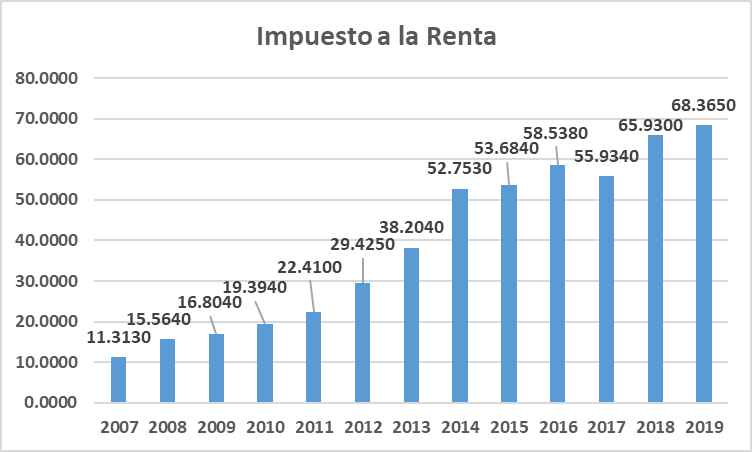
\includegraphics{20230603225440.png}

}

\end{figure}

Interpretación:

La figura muestra la recaudación interna de impuestos a la renta por
parte de la SUNAT en el departamento de Ayacucho. Se observa un claro
crecimiento a lo largo de los años, pasando de 11,313 miles de soles en
2007 a 68,365 miles de soles en 2019. Sin embargo, en 2017 se registró
una disminución en la recaudación de impuestos a la renta en comparación
con el año anterior. Esta caída se debe principalmente a las menores
recaudaciones en los impuestos de segunda categoría, tercera categoría y
cuarta categoría.

\begin{figure}

\caption{\label{fig-2}Ayacucho: Impuesto General a las ventas (IGV) 2007
- 2019 (Milesde S/).}

{\centering 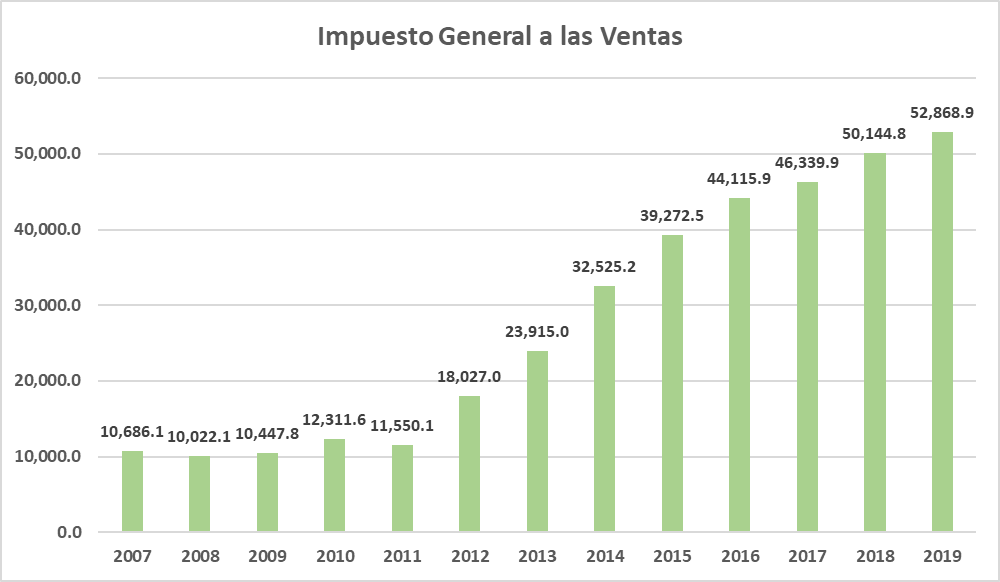
\includegraphics{20230603225447.png}

}

\end{figure}

Nota: Incluye el Impuesto General a las Ventas por Cuenta Propia, No
Domiciliados y liquidaciones de compra-retenciones, operaciones internas
arroz, Impuesto Especial a las Ventas, Decreto de Urgencia N°
089-97(DCTP Fertilizantes) e Impuesto Promoción Municipal.

Interpretación:

El impuesto general a las ventas es una de las principales fuentes de
recaudación en el departamento de Ayacucho. Durante el período
estudiado, se observó un importante crecimiento en esta recaudación,
como se muestra en la figura. Pasó de 10,686.1 miles de soles en 2007 a
52,868.9 miles de soles en 2019, alcanzando su punto máximo de
recaudación en este último año. Aunque se registraron algunas caídas
leves en los años 2019 y 2011, en general, el impuesto general a las
ventas mostró un crecimiento significativo hasta 2019.

\begin{figure}

\caption{\label{fig-3}Ayacucho: Impuesto Selectivo al consumo (ISC) 2007
- 2019 (Miles de s/).}

{\centering 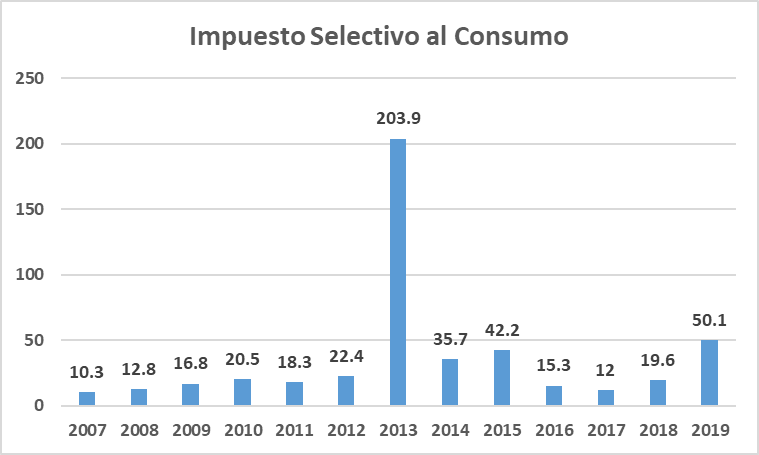
\includegraphics{20230603225455.png}

}

\end{figure}

Nota: Incluye combustibles, gaseosas, cervezas, cigarrillos,
tragamonedas, licores, agua mineral, vehículos, pagos de I.S.C. en
formularios 151 y 185, Casinos de juego, Juegos de azar y apuestas,
Loterías, Bingos, Rifas y Eventos hípicos.

Interpretación:

Aunque el impuesto selectivo al consumo (ISC) es uno de los sectores de
menor recaudación en el departamento de Ayacucho, la tabla muestra un
crecimiento significativo a lo largo de los años. En 2007, la
recaudación por este concepto fue de solo 10.3 mil soles, pero en 2017
superó los 203.9 mil soles, siendo la cifra más alta entre los periodos
mencionados. A pesar de su posición relativamente baja en comparación
con otros impuestos, el ISC experimentó un notorio incremento a lo largo
del tiempo en el departamento de Ayacucho.

\hypertarget{crecimiento-econuxf3mico-del-departamento-de-ayacucho-en-el-periodo-2007-2019}{%
\subsubsection{Crecimiento económico del departamento de Ayacucho en el
periodo 2007 --
2019}\label{crecimiento-econuxf3mico-del-departamento-de-ayacucho-en-el-periodo-2007-2019}}

\hypertarget{tbl-3}{}
\begin{longtable}[]{@{}
  >{\raggedright\arraybackslash}p{(\columnwidth - 26\tabcolsep) * \real{0.0714}}
  >{\raggedright\arraybackslash}p{(\columnwidth - 26\tabcolsep) * \real{0.0714}}
  >{\raggedright\arraybackslash}p{(\columnwidth - 26\tabcolsep) * \real{0.0714}}
  >{\raggedright\arraybackslash}p{(\columnwidth - 26\tabcolsep) * \real{0.0714}}
  >{\raggedright\arraybackslash}p{(\columnwidth - 26\tabcolsep) * \real{0.0714}}
  >{\raggedright\arraybackslash}p{(\columnwidth - 26\tabcolsep) * \real{0.0714}}
  >{\raggedright\arraybackslash}p{(\columnwidth - 26\tabcolsep) * \real{0.0714}}
  >{\raggedright\arraybackslash}p{(\columnwidth - 26\tabcolsep) * \real{0.0714}}
  >{\raggedright\arraybackslash}p{(\columnwidth - 26\tabcolsep) * \real{0.0714}}
  >{\raggedright\arraybackslash}p{(\columnwidth - 26\tabcolsep) * \real{0.0714}}
  >{\raggedright\arraybackslash}p{(\columnwidth - 26\tabcolsep) * \real{0.0714}}
  >{\raggedright\arraybackslash}p{(\columnwidth - 26\tabcolsep) * \real{0.0714}}
  >{\raggedright\arraybackslash}p{(\columnwidth - 26\tabcolsep) * \real{0.0714}}
  >{\raggedright\arraybackslash}p{(\columnwidth - 26\tabcolsep) * \real{0.0714}}@{}}
\caption{\label{tbl-3}Valor Agregado Bruto (VAB) según actividad
económica en Ayacucho (2007-2019, Tasa de crecimiento
\%)}\tabularnewline
\toprule\noalign{}
\begin{minipage}[b]{\linewidth}\raggedright
Actividades
\end{minipage} & \begin{minipage}[b]{\linewidth}\raggedright
2007
\end{minipage} & \begin{minipage}[b]{\linewidth}\raggedright
2008
\end{minipage} & \begin{minipage}[b]{\linewidth}\raggedright
2009
\end{minipage} & \begin{minipage}[b]{\linewidth}\raggedright
2010
\end{minipage} & \begin{minipage}[b]{\linewidth}\raggedright
2011
\end{minipage} & \begin{minipage}[b]{\linewidth}\raggedright
2012
\end{minipage} & \begin{minipage}[b]{\linewidth}\raggedright
2013
\end{minipage} & \begin{minipage}[b]{\linewidth}\raggedright
2014
\end{minipage} & \begin{minipage}[b]{\linewidth}\raggedright
2015
\end{minipage} & \begin{minipage}[b]{\linewidth}\raggedright
2016
\end{minipage} & \begin{minipage}[b]{\linewidth}\raggedright
2017
\end{minipage} & \begin{minipage}[b]{\linewidth}\raggedright
2018
\end{minipage} & \begin{minipage}[b]{\linewidth}\raggedright
2019
\end{minipage} \\
\midrule\noalign{}
\endfirsthead
\toprule\noalign{}
\begin{minipage}[b]{\linewidth}\raggedright
Actividades
\end{minipage} & \begin{minipage}[b]{\linewidth}\raggedright
2007
\end{minipage} & \begin{minipage}[b]{\linewidth}\raggedright
2008
\end{minipage} & \begin{minipage}[b]{\linewidth}\raggedright
2009
\end{minipage} & \begin{minipage}[b]{\linewidth}\raggedright
2010
\end{minipage} & \begin{minipage}[b]{\linewidth}\raggedright
2011
\end{minipage} & \begin{minipage}[b]{\linewidth}\raggedright
2012
\end{minipage} & \begin{minipage}[b]{\linewidth}\raggedright
2013
\end{minipage} & \begin{minipage}[b]{\linewidth}\raggedright
2014
\end{minipage} & \begin{minipage}[b]{\linewidth}\raggedright
2015
\end{minipage} & \begin{minipage}[b]{\linewidth}\raggedright
2016
\end{minipage} & \begin{minipage}[b]{\linewidth}\raggedright
2017
\end{minipage} & \begin{minipage}[b]{\linewidth}\raggedright
2018
\end{minipage} & \begin{minipage}[b]{\linewidth}\raggedright
2019
\end{minipage} \\
\midrule\noalign{}
\endhead
\bottomrule\noalign{}
\endlastfoot
Agricultura, Ganadería, Caza y Silvicultura & 3.3 & 14.3 & 3.2 & -5.1 &
-4.1 & 16.1 & -5.3 & -9.2 & 1.3 & -1.2 & 6.1 & 15.2 & -1.3 \\
Pesca y Acuicultura & -13.4 & -18.5 & 10.8 & -7.7 & 121.7 & 37.4 & 2.3 &
5.5 & 13.6 & 12.1 & 41.9 & 1.9 & -51.7 \\
Extracción de Petróleo, Gas y Minerales & 107.4 & 49.6 & 35.8 & 6.2 &
3.3 & 2.7 & 25.9 & -3.1 & 14.8 & -0.8 & 6.4 & 3.4 & 6.2 \\
Manufactura & 6.7 & 6.0 & 0.2 & 7.4 & 4.4 & 2.0 & -0.3 & -7.9 & -2.4 &
3.7 & 2.1 & 5.6 & 0.1 \\
Electricidad, Gas y Agua & 2.1 & 7.4 & -1.6 & 8.1 & 5.6 & 10.8 & 6.1 &
15.2 & 7.0 & -18.2 & 4.9 & 6.3 & 0.5 \\
Construcción & 36.6 & 10.9 & 14.2 & 12.3 & 21.8 & 23.9 & 26.4 & 0.3 &
2.2 & -15.5 & 11.0 & 7.7 & -1.1 \\
Comercio & 6.7 & 12.6 & 2.3 & 10.1 & 6.8 & 13.2 & 6.1 & 1.0 & 1.9 & 1.6
& 1.1 & 1.4 & 2.4 \\
Transporte, Almacenamiento, Correo y Mensajería & 10.7 & 8.2 & 2.5 & 8.2
& 8.5 & 7.0 & 6.0 & 3.7 & 3.5 & 3.3 & 2.9 & 2.6 & 2.2 \\
Alojamiento y Restaurantes & 8.5 & 9.9 & 0.6 & 5.6 & 8.5 & 9.0 & 6.9 &
4.2 & 2.8 & 3.2 & 2.0 & 4.0 & 4.8 \\
Telecomunicaciones y Otros Servicios de Información & 0 & 24.5 & 14.3 &
15.9 & 15.0 & 17.9 & 14.1 & 11.0 & 10.1 & 13.8 & 12.4 & 9.8 & 7.8 \\
Administración Pública y Defensa & 4.7 & 7.5 & 13.2 & 2.9 & 3.8 & 4.0 &
4.0 & 4.6 & 6.6 & 7.6 & 5.4 & 5.7 & 6.0 \\
Otros Servicios & 6.9 & 3.9 & 5.2 & 3.7 & 5.0 & 6.7 & 5.8 & 5.7 & 6.0 &
4.6 & 3.7 & 3.6 & 2.9 \\
Valor Agregado Bruto & 12.3 & 14.3 & 10.3 & 4.6 & 4.8 & 9.0 & 9.4 & -0.5
& 5.8 & 0.3 & 5.3 & 5.6 & 2.9 \\
\end{longtable}

Fuente: Elaboración propia (datos: INEI, BCRP)

\begin{figure}

\caption{\label{fig-4}Ayacucho: Valor agregado Bruto (VAB) según
actividad económica 2007-2019 (Tasa de crecimiento, \%)}

{\centering 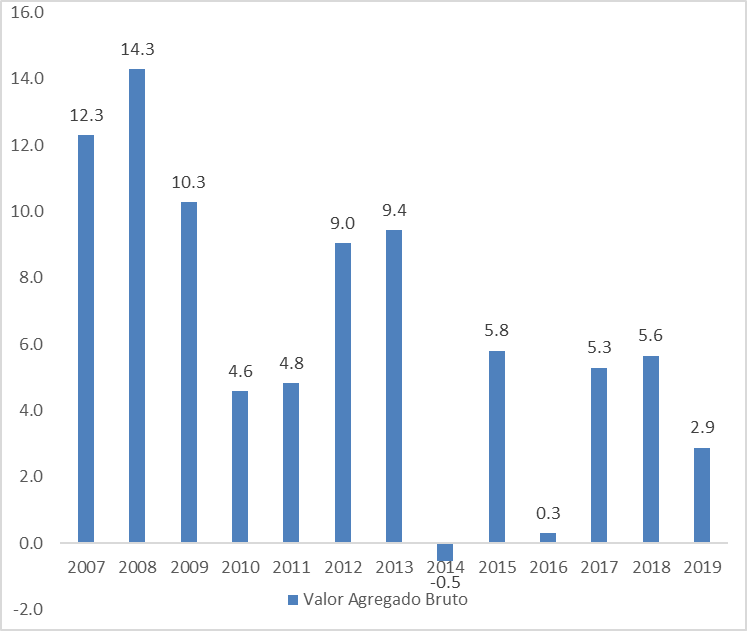
\includegraphics{20230603230848.png}

}

\end{figure}

La evolución del Valor Agregado Bruto (VAB) en la región de Ayacucho se
muestra en el gráfico, revelando variaciones significativas a lo largo
de los últimos años. Aunque no se observa un crecimiento continuo, se
destaca que en algunos períodos el VAB ha experimentado un crecimiento
negativo, como en el año 2014 con una disminución del 0.5\%. Es
importante mencionar que el año más destacado en términos de crecimiento
fue el 2008, cuando alcanzó un impresionante incremento del 14.3\%.

\hypertarget{relaciuxf3n-entre-el-crecimiento-econuxf3mico-y-la-recaudaciuxf3n-de-impuestos-en-la-sunat-departamento-de-lambayeque-en-el-periodo-2007-2019}{%
\subsubsection{Relación entre el crecimiento económico y la recaudación
de impuestos en la SUNAT, departamento de Lambayeque en el periodo 2007
--
2019}\label{relaciuxf3n-entre-el-crecimiento-econuxf3mico-y-la-recaudaciuxf3n-de-impuestos-en-la-sunat-departamento-de-lambayeque-en-el-periodo-2007-2019}}

Nuestro objetivo es analizar la relación entre el crecimiento económico
y la recaudación de impuestos en el departamento de Ayacucho. Utilizamos
como indicador de crecimiento económico la actividad económica de la
región y la recaudación de impuestos por parte de la SUNAT. Para
lograrlo, aplicamos estimaciones econométricas lineales mediante un
modelo de regresión lineal simple. El propósito de este enfoque es
demostrar el efecto del crecimiento económico en la recaudación de
impuestos. Los parámetros estimados en el modelo son los siguientes:

Modelo: \(R_i = \beta_{1} + \beta_{2}VAB + \mu_{i}\)

Dependent Variable: RI

Method: Least Squares

Date: 12/27/21 Time: 19:06

Sample: 2007-2019

Included observations: 13

\hypertarget{tbl-4}{}
\begin{longtable}[]{@{}
  >{\raggedright\arraybackslash}p{(\columnwidth - 8\tabcolsep) * \real{0.2000}}
  >{\raggedright\arraybackslash}p{(\columnwidth - 8\tabcolsep) * \real{0.2000}}
  >{\raggedright\arraybackslash}p{(\columnwidth - 8\tabcolsep) * \real{0.2000}}
  >{\raggedright\arraybackslash}p{(\columnwidth - 8\tabcolsep) * \real{0.2000}}
  >{\raggedright\arraybackslash}p{(\columnwidth - 8\tabcolsep) * \real{0.2000}}@{}}
\caption{\label{tbl-4}Resultados del modelo estimado
inicial}\tabularnewline
\toprule\noalign{}
\begin{minipage}[b]{\linewidth}\raggedright
Variable
\end{minipage} & \begin{minipage}[b]{\linewidth}\raggedright
Coefficient
\end{minipage} & \begin{minipage}[b]{\linewidth}\raggedright
Std. Error
\end{minipage} & \begin{minipage}[b]{\linewidth}\raggedright
t-Statistic
\end{minipage} & \begin{minipage}[b]{\linewidth}\raggedright
Prob.
\end{minipage} \\
\midrule\noalign{}
\endfirsthead
\toprule\noalign{}
\begin{minipage}[b]{\linewidth}\raggedright
Variable
\end{minipage} & \begin{minipage}[b]{\linewidth}\raggedright
Coefficient
\end{minipage} & \begin{minipage}[b]{\linewidth}\raggedright
Std. Error
\end{minipage} & \begin{minipage}[b]{\linewidth}\raggedright
t-Statistic
\end{minipage} & \begin{minipage}[b]{\linewidth}\raggedright
Prob.
\end{minipage} \\
\midrule\noalign{}
\endhead
\bottomrule\noalign{}
\endlastfoot
C & -135238.1 & 18103.46 & -7.470290 & 0.0000 \\
VAB & 0.046999 & 0.003858 & 12.18173 & 0.0000 \\
R-squared & 0.930989 & Mean dependent var & 81344.83 & \\
Adjusted R-squared & 0.924715 & S.D. dependent var & 44814.89 & \\
S.E. of regression & 12296.35 & Akaike info criterion & 21.81263 & \\
Sum squared resid & 1.66E+09 & Schwarz criterion & 21.89955 & \\
Log likelihood & -139.7821 & Hannan-Quinn criter. & 21.79477 & \\
F-statistic & 148.3945 & Durbin-Watson stat & 0.880483 & \\
Prob(F-statistic) & 0.000000 & & & \\
\end{longtable}

La variable independiente del PBI departamental explica el 93.1\% de la
variabilidad de los impuestos, con un total de 13 observaciones. Según
la prueba de t de Student, los parámetros del modelo son
estadísticamente significativos con un nivel de significancia del 5\%.
Además, de acuerdo a la prueba F, el modelo es estadísticamente
significativo.

Para analizar la estacionariedad de las variables, se utilizó el
\textbf{test de Dickey-Fuller aumentado}, el cual es ampliamente
empleado en la literatura. Se aplicó este test a la serie de logaritmo
de la variable VAB con su diferencia, utilizando el criterio de
información de Akaike. El valor crítico obtenido fue de -1.91, el cual
es menor que -2.86 con un nivel de significancia del 5\%. Por lo tanto,
se acepta la hipótesis nula, lo que implica la existencia de raíz
unitaria y no estacionariedad (Anexo-Figura 5).

Se realizó el mismo análisis de estacionariedad utilizando el test de
Dickey-Fuller aumentado para la variable RI. Se obtuvo un valor crítico
de -0.057, el cual es menor que -2.86 con un nivel de significancia del
5\%. Por lo tanto, se acepta la hipótesis nula, indicando la existencia
de raíz unitaria y no estacionalidad (Anexo-Figura 6).

Se aplicó la \textbf{prueba de Phillips Perron} a nuestra variable
independiente, obteniendo un p-valor de -1.75 con un nivel de
significancia del 5\%. Se acepta la hipótesis nula, lo que indica la
existencia de raíz unitaria y no estacionariedad (Anexo-Figura 7).
También se realizó la prueba de Phillips Perron para la variable
dependiente, obteniendo un p-valor de 0.056 con un nivel de
significancia del 5\%. Se acepta la hipótesis nula, lo que sugiere la
existencia de raíz unitaria y no estacionariedad (Anexo-Figura 8).

Para detectar la presencia de \textbf{heterocedasticidad} en los
errores, se llevaron a cabo dos pruebas: la prueba de White y la prueba
Koenker-Bassett. En ambos casos, se concluyó que no hay evidencia de
heterocedasticidad en nuestra regresión (Anexo-Figuras 11 y 12).

Se realizó una \textbf{prueba de autocorrelación} utilizando el
estadístico Durbin-Watson. Un valor de d menor que 1.01 o mayor que 2.99
indica un problema potencialmente grave de autocorrelación. En nuestro
caso, el estadístico Durbin-Watson es 0.8880485, que es menor que 1.5,
lo que indica la presencia de problemas de autocorrelación
(Anexo-Figuras 13 y 14).

Se llevó a cabo un análisis de causalidad utilizando la \textbf{prueba
de Granger} para examinar las combinaciones de las variables de
recaudación de impuestos y Valor Agregado Bruto (VAB). El resultado de
la prueba de causalidad de Granger muestra un p-valor menor que 0.05, lo
cual nos lleva a rechazar la hipótesis nula de que el VAB causa cambios
en la recaudación de impuestos. Para determinar el rezago óptimo, se
utilizó el criterio de información de Akaike, y se encontró que el
primer rezago era el más adecuado (Anexo-Figura 9).

\hypertarget{discusiuxf3n-de-los-resultados}{%
\section{Discusión de los
Resultados}\label{discusiuxf3n-de-los-resultados}}

El crecimiento económico, representado por el Valor Agregado Bruto
(VAB), es fundamental para los gobiernos, ya que el gobierno busca
alcanzar un crecimiento óptimo y estable en la producción. En esta
investigación, se evaluó el crecimiento económico del departamento de
Ayacucho durante el periodo 2007-2019, centrándose en los sectores
productivos como indicadores de dicho crecimiento. Los resultados
mostraron que el crecimiento económico del departamento de Ayacucho tuvo
un impacto positivo en los ingresos generados por los impuestos,
destacando la contribución más significativa del Impuesto General a la
Renta. Además, se identificó que la evasión tributaria influye en la
recaudación de impuestos.

El crecimiento económico puede influir en una mayor recaudación
tributaria, por lo que el objetivo de esta investigación fue analizar la
relación entre ambas variables. Los resultados revelaron una relación
casi perfecta entre el crecimiento económico y la recaudación de
impuestos. Mediante el uso de una regresión lineal y un análisis
estadístico, se obtuvo un coeficiente de determinación del 93.1\%, lo
que indica que la variable independiente del PBI departamental explica
de manera significativa la variable dependiente de la recaudación de
impuestos. Además, se verificó la significancia estadística de los
parámetros del modelo mediante la prueba de t de Student con un nivel de
significancia del 5\%. Asimismo, la prueba F confirmó que el modelo es
estadísticamente significativo.

\hypertarget{conclusiones}{%
\section{Conclusiones}\label{conclusiones}}

En conclusión, el análisis estadístico de causalidad de las variables
demuestra que el Valor Agregado Bruto (VAB) es un factor determinante en
la recaudación de impuestos en el departamento de Ayacucho durante el
periodo 2007-2019.

En cuanto a la recaudación de impuestos en Ayacucho, se observa un
notable crecimiento del 4.02\% en 2012, impulsado por un crecimiento
económico del 0.53\%. Sin embargo, se registró una brusca caída del
0.05\% en la recaudación de impuestos en 2017, debido a una disminución
del Valor Agregado Bruto por debajo de su línea de tendencia, algo que
no había ocurrido desde 2007.

El Valor Agregado Bruto experimentó un crecimiento acelerado desde 2008
hasta 2015, pero a partir de ese año su crecimiento se situó por debajo
de la línea de tendencia. A pesar de ello, se observó un incremento en
la recaudación fiscal.

Por otro lado, mediante una regresión lineal simple se estableció el
grado de asociación o relación entre las variables. Se encontró que la
recaudación de impuestos muestra un coeficiente de 0.046, lo que
significa que un aumento del 1\% en el Valor Agregado Bruto se traduce
en un incremento del 4.6\% en la recaudación de impuestos en el
departamento de Ayacucho. Esto demuestra que la recaudación de impuestos
es sensible al crecimiento económico.

\hypertarget{referencias}{%
\section{Referencias}\label{referencias}}

\printbibliography[heading=none]




\end{document}
